\chapter{Cosmology for the Data Analyst}\label{ch:T1}

\providecommand{\TOneLmax}{}\renewcommand{\TOneLmax}{2500}
\providecommand{\TOneCosAsTauTT}{}\renewcommand{\TOneCosAsTauTT}{-0.999}
\providecommand{\TOneCosAsTauEElow}{}\renewcommand{\TOneCosAsTauEElow}{0.98}
\providecommand{\TOneAsRespHigh}{}\renewcommand{\TOneAsRespHigh}{1.41}
\providecommand{\TOneTauRespHigh}{}\renewcommand{\TOneTauRespHigh}{-1.46}
\providecommand{\TOneTauRespEElow}{}\renewcommand{\TOneTauRespEElow}{46}
\providecommand{\TOneNsPivotEll}{}\renewcommand{\TOneNsPivotEll}{542}
\providecommand{\TOneMaxRespOmc}{}\renewcommand{\TOneMaxRespOmc}{1.1}
\providecommand{\TOneDpeakEll}{}\renewcommand{\TOneDpeakEll}{220}
\providecommand{\TOneDpeak}{}\renewcommand{\TOneDpeak}{5732}
\providecommand{\TOneSigmaEight}{}\renewcommand{\TOneSigmaEight}{0.8111}
\providecommand{\TOneSigmaEightOurs}{}\renewcommand{\TOneSigmaEightOurs}{0.8112}
\providecommand{\TOneSigmaEightZone}{}\renewcommand{\TOneSigmaEightZone}{0.4928}
\providecommand{\TOneRdrag}{}\renewcommand{\TOneRdrag}{147.10}
\providecommand{\TOneRdragH}{}\renewcommand{\TOneRdragH}{99.1}
\providecommand{\TOneRpeak}{}\renewcommand{\TOneRpeak}{101.5}
\providecommand{\TOneKnl}{}\renewcommand{\TOneKnl}{0.15}
\providecommand{\TOneKnlZone}{}\renewcommand{\TOneKnlZone}{0.21}
\providecommand{\TOneKpeak}{}\renewcommand{\TOneKpeak}{0.017}
\providecommand{\TOneRatioOne}{}\renewcommand{\TOneRatioOne}{5.9}
 
\section*{Where this chapter is going}
\addcontentsline{toc}{section}{Where this chapter is going}
\label{T1a:sec:roadmap}

A cosmological model is a machine. We feed it six numbers, and it returns the \emph{statistics} of the sky: the angular power spectrum $\Cell$ of the microwave background (how much the temperature varies on each angular scale), the matter power spectrum $P(k)$ (the same for the matter density, scale by scale), and the distance to every redshift. CAMB \cite{CAMB2000} is that machine in code. The machine never returns the sky itself. Our sky, with its particular hot and cold spots and its particular galaxies, is one noisy draw from the statistics the machine predicts. Every later chapter works across that gap. The model predicts a distribution. The data are one draw from it. Statistics is how we read the six numbers back from that one draw.

The book follows one pipeline (\cref{ch:00}): a theory, its data, a compressed statistic, that statistic's scatter, and back to the theory. Cosmology is the first step. It fixes what each summary \emph{should} be on average. The physics behind each object is worked out in the cosmology notes. The data analyst needs less: which objects the statistics uses, what each one means in one line, the equation that defines it, where CAMB and the cosmology notes write it differently, and how the predicted statistics move when the six numbers move. \Cref{T1a:fig:roadmap} is the map.

\begin{figure}[htbp]
\centering
\begin{tikzpicture}[
  box/.style={draw=accent,rounded corners=2pt,fill=ideabg,align=center,font=\small,
              minimum width=3.1cm,minimum height=1.0cm,inner sep=3pt},
  obox/.style={box,minimum width=3.3cm,draw=formblue},
  dat/.style={box,fill=warnbg,draw=bdryred,minimum width=3.6cm},
  arr/.style={->,thick,accent},
  note/.style={font=\scriptsize,softgray,align=center}]
  \node[box] (par) at (0,0) {six numbers $\params$\\ $\Omega_{b0}h^2,\ \Omega_{c0}h^2,\ H_0$\\ $\tau,\ A_s,\ n_s$};
  \node[box] (camb) at (3.9,0) {CAMB\\ background $E(z)$,\\ transfer functions};
  \node[obox] (dist) at (8.3,1.5) {distances\\ $D_A(z),\ D_L(z),\ H(z)$};
  \node[obox] (cmb)  at (8.3,0) {CMB spectra\\ $\Cell$, $D_\ell$, lensing};
  \node[obox] (mat)  at (8.3,-1.5) {matter\\ $P(k)$, $\xi(r)$, $\sigma_8$};
  \node[draw=formblue,dashed,rounded corners=3pt,inner sep=5pt,fit=(dist)(cmb)(mat)] (pred) {};
  \draw[arr] (par) -- (camb);
  \draw[arr] (camb.east) -- (dist.west);
  \draw[arr] (camb.east) -- (cmb.west);
  \draw[arr] (camb.east) -- (mat.west);
  \node[dat] (sky) at (8.3,-3.9) {\textit{nature draws once:}\\ SN magnitudes, $\alm$ of our sky,\\ galaxy positions};
  \node[box,fill=takebg,draw=tangentgreen] (inf) at (3.9,-3.9) {\textit{inference:}\\ likelihood, MCMC,\\ Fisher, topology};
  \draw[arr,bdryred] (pred.south) -- (sky.north);
  \draw[arr,tangentgreen] (sky) -- (inf);
  \draw[arr,tangentgreen,dashed] (inf.west) -| (par.south);
\end{tikzpicture}
\caption{The machine and its one output we can see. Six numbers go into CAMB, which returns three families of predicted statistics (blue). Nature does not hand us those statistics: it hands us a single noisy draw from them (red), and the statistics of the later chapters (green) turn that draw back into constraints on the six numbers.}
\label{T1a:fig:roadmap}
\end{figure}

The link between the cosmology and the statistics is how the outputs move when the inputs move. Nudge one parameter and watch $\Cell$ respond. That response is a derivative, and the Fisher matrix of \cref{ch:10} is built from such derivatives. If two parameters produce responses that look alike, the data cannot tell those parameters apart. This is a degeneracy, and the MCMC chains of \cref{ch:09} show it as a long ridge. On the matter side, the linear $P(k)$ is the input of the Gaussian random fields of \cref{ch:07}. On small scales gravity makes the real spectrum (computed by the halofit recipe) depart from the linear one. There the field is no longer Gaussian, and the topological summaries of \cref{ch:12} have something to find that the power spectrum misses.

\section{Six numbers in, statistics out}
\label{T1a:sec:machine}

Think of the flat $\Lambda$CDM model as a function with six inputs.
Two inputs are physical densities: the baryon density $\Omega_{b0}h^2$ and the cold dark matter density $\Omega_{c0}h^2$ \unpack{today's density of each component divided by the critical density, times $h^2$; the product is a physical density that does not depend on $H_0$}.
One input fixes the distances: either the Hubble constant $H_0=100\,h\ \mathrm{km\,s^{-1}\,Mpc^{-1}}$, or equivalently the angle $\theta_{\mathrm{MC}}$ that the sound horizon at decoupling subtends on the sky.
One is the optical depth to reionisation, $\tau$ \unpack{the expected number of Thomson scatterings a CMB photon undergoes after the Universe is re-ionised; a fraction $e^{-\tau}$ of the photons arrive unscattered}.
The last two describe the primordial fluctuations: their amplitude $A_s$ and their spectral tilt $n_s$.
Everything else is held fixed: the radiation density (from the measured CMB temperature), flatness $\Omega_{K0}=0$, and a single massive neutrino of $0.06$\,eV.

These numbers appear in three places, and \cref{T1a:tab:params} translates between them: the symbol used in the cosmology notes, the keyword that CAMB's Python interface takes, and the Planck 2018 value with its 68\% error \cite[Table~1]{Planck2018VI}. The book's fiducial model (\pyname{code/camb_fiducial.py}) is this best fit. The $\pm1\sigma$ errors are the step sizes of the first experiment (\cref{T1a:sec:cl-response}).

\begin{table}[htbp]
\centering
\small
\renewcommand{\arraystretch}{1.2}
\begin{tabularx}{\linewidth}{@{}>{\raggedright\arraybackslash}p{2.6cm}
                               >{\raggedright\arraybackslash}X
                               >{\raggedright\arraybackslash}p{2.55cm}
                               >{\raggedright\arraybackslash}p{3.3cm}@{}}
\toprule
symbol (cosmology notes) & one-line meaning & CAMB keyword & Planck 2018 (68\%)\\\midrule
$\Omega_{b0}h^2$ & physical baryon density; sets the baryon loading of the acoustic oscillations & \pyname{ombh2} & $0.02237\pm0.00015$\\
$\Omega_{c0}h^2$ & physical cold dark matter density; sets matter--radiation equality & \pyname{omch2} & $0.1200\pm0.0012$\\
$100\,\theta_{\mathrm{MC}}$ \emph{or} $H_0$ & angular size of the sound horizon at decoupling, or the expansion rate today & \pyname{cosmomc_theta} or \pyname{H0} & $1.04092\pm0.00031$; $H_0=67.36\pm0.54$ (derived)\\
$\tau$ & optical depth to reionisation & \pyname{tau} & $0.0544\pm0.0073$\\
$A_s$ & amplitude of the primordial curvature spectrum at $k_*=0.05\,\mathrm{Mpc}^{-1}$ & \pyname{As} & $\ln(10^{10}A_s)=3.044\pm0.014$\\
$n_s$ & tilt of that spectrum, $n_s=1$ being scale invariant & \pyname{ns} & $0.9649\pm0.0042$\\
\bottomrule
\end{tabularx}
\caption{The six $\Lambda$CDM numbers in three notations. Planck samples $\theta_{\mathrm{MC}}$ because the data measure that angle almost directly; CAMB is usually called with $H_0$ instead, and the book's scripts do so (CAMB's \pyname{cosmomc_theta} takes $\theta_{\mathrm{MC}}$ itself, not $100\,\theta_{\mathrm{MC}}$). The error on $\ln(10^{10}A_s)$ is the fractional error on $A_s$, $1.4\%$.}
\label{T1a:tab:params}
\end{table}

The machine's output is a set of averages, not a sky. This is the one idea from cosmology that the statistics cannot do without. Take the CMB. Write the temperature pattern of the sky as a sum of spherical harmonics $Y_{\ell m}$; the coefficient of each one is a number $\alm$, and large $\ell$ means small angular scales. What does the model predict about these numbers? It predicts a definite value for $\Cell$, the average of $\abs{\alm}^2$, computed from the primordial power spectrum and the radiation transfer function. It never predicts any single $\alm$. Each $\alm$ of our sky is one random draw from a distribution of variance $\Cell$. The matter field works the same way: the model predicts $P(k)$, the variance of each Fourier mode of the matter density, and not the modes themselves. So comparing theory with data always means comparing a predicted \emph{distribution} with one \emph{draw}. A single draw scatters about its mean, and nothing can remove that scatter, because we have only one sky. That scatter is cosmic variance.

\begin{keyidea}[What the model predicts]
A cosmological model predicts the statistics of the fields (their power spectra, correlation functions and distances), never the fields themselves. The observed sky is one realisation. Every estimator in the later chapters is a function of that realisation, and its sampling distribution around the predicted statistic is what the likelihood describes.
\end{keyidea}

\section{The objects the statistics uses}
\label{T1a:sec:objects}

A revision of the cosmology a data analyst needs follows the order in which the machine of \cref{T1a:sec:machine} works. First comes the smooth background, the expansion of the Universe and the distances that follow from it. Then the primordial seed and how the radiation and matter eras process it. Last come the statistics of the two fields that result, the temperature of the sky and the density of matter. For every object the question comes first, then the equation it starts from and the working equation the book uses, then the size of the thing, then the chapters that use it. The physics between the two equations is worked out in the cosmology notes. Here it is a sentence.

\paragraph{How fast the Universe expands: $H(z)$ and $E(z)$.}
The question is how the expansion rate $H$ changed over cosmic history, because every distance below is built from it. A homogeneous, isotropic universe has the Friedmann--Lema\^itre--Robertson--Walker metric, with one function of time in it, the scale factor $a(t)$. Einstein's equations then reduce to the first Friedmann equation
\begin{equation*}
H^2\equiv\Bigl(\frac{\dot a}{a}\Bigr)^2=\frac{8\pi G}{3}\rho-\frac{K}{a^2}+\frac{\Lambda}{3},
\end{equation*}
where $\rho$ is the total density of radiation and matter, $K$ the spatial curvature and $\Lambda$ the cosmological constant. Each component dilutes in its own way as space expands: radiation as $a^{-4}$ (the photons also lose energy), matter as $a^{-3}$, curvature as $a^{-2}$, and $\Lambda$ not at all. Write the redshift as $1+z=a_0/a$ and divide by today's rate $H_0$. The result is the working equation, in terms of the dimensionless expansion rate $E(z)\equiv H(z)/H_0$:
\begin{equation*}
E^2(z)=\Omega_{r0}(1+z)^4+\Omega_{m0}(1+z)^3+\Omega_{K0}(1+z)^2+\Omega_{\Lambda0},
\qquad
\Omega_{K0}=1-\Omega_{m0}-\Omega_{r0}-\Omega_{\Lambda0}.
\end{equation*}
The $\Omega_{X0}$ are today's densities as fractions of the critical density $3H_0^2/8\pi G$, with $X=r$ for radiation, $m$ for matter, $K$ for curvature and $\Lambda$ for the cosmological constant, and the second relation says that the fractions add up to one. For the Planck fit, $\Omega_{m0}\approx0.315$, $\Omega_{\Lambda0}\approx0.685$, $\Omega_{r0}\approx9\times10^{-5}$ and $\Omega_{K0}\approx0$. The matter term wins over the others at $z\gtrsim0.3$, and radiation beats matter only for $z\gtrsim3000$. Today's numbers are $E(1)\approx1.79$, so the Universe expanded $1.8$ times faster at $z=1$. Of the six parameters of \cref{T1a:tab:params}, the data fix not $\Omega_{m0}$ itself but the physical density $\Omega_{m0}h^2=\Omega_{b0}h^2+\Omega_{c0}h^2\,(+\Omega_{\nu0}h^2)\approx0.143$, which is what the expansion history before the epoch of dark energy depends on. This is the model mean of the supernova and BAO data of \cref{ch:03,ch:05}, and the matter density is what the fits of \cref{ch:09,ch:10} constrain.

\paragraph{How far away is a source: $D_C$, $D_M$, $D_A$ and $D_L$.}
The question is what ``distance'' means for an object at redshift $z$, because the same source has a different distance depending on whether we measure it with a ruler or a candle. A light ray travels along a null path, $c\,\dd t=a\,\dd\chi$ in terms of the comoving radial coordinate $\chi$, and $\dd z=-(1+z)H\,\dd t$. Integrating along the ray from the source to us gives the comoving distance, with the Hubble distance $D_{H0}\equiv c/H_0$ as the unit:
\begin{equation*}
a_0\chi(z)=D_{H0}\int_0^{z}\frac{\dd z'}{E(z')} .
\end{equation*}
Curvature bends the ray's transverse separation, so the comoving transverse distance is $a_0f_K[\chi(z)]$, where $f_K(\chi)=\chi$ in a flat universe and is a $\sin$ or $\sinh$ of $\chi$ in a closed or open one. A source of physical size $s$ at redshift $z$ subtends the angle $\vartheta=s/D_A$ with the angular-diameter distance, and a source of luminosity $L$ gives the flux $F=L/4\pi D_L^2$ with the luminosity distance:
\begin{equation*}
D_A(z)=\frac{a_0f_K[\chi(z)]}{1+z},
\qquad
D_L(z)=(1+z)^2D_A(z).
\end{equation*}
The first divides by $1+z$ because the source was closer to us when the light left it, and the second multiplies by $(1+z)^2$ because redshift costs each photon energy and stretches the arrival rate. The Hubble distance is $D_{H0}=c/H_0\approx4450$\,Mpc. For the Planck model, a source at $z=1$ has comoving distance $3.4$\,Gpc, $D_A=1.7$\,Gpc and $D_L=6.8$\,Gpc, and the last-scattering surface at $z\approx1090$ is $13.9$\,Gpc away. Note that $D_A$ does not grow forever: it peaks near $1.8$\,Gpc at $z\approx1.6$ and then falls, so a rod at high redshift looks larger on the sky. Supernova magnitudes depend on $D_L(z)$, and the BAO ruler of the next paragraph on $D_A(z)$ and $H(z)$ (\cref{ch:03,ch:05}).

\paragraph{The acoustic ruler: the sound horizon $r_s$.}
The question is how far a sound wave could travel in the early plasma, because that length is a ruler that the CMB calibrates. Before recombination photons and baryons were locked into one fluid. A pressure wave in it moves at the sound speed $c_s=c/\sqrt{3(1+R)}$, which is the radiation value $c/\sqrt3$ slowed down by the baryons' inertia. Here $R\equiv3\rho_b/(4\rho_\gamma)$ is the baryon-to-photon momentum ratio, a number of order $0.6$ at the drag epoch. The distance such a wave covers up to conformal time $\eta$ is
\begin{equation*}
r_s(\eta)\equiv\int_0^\eta c_s\,\dd\eta'=\int_0^\eta\frac{c\,\dd\eta'}{\sqrt{3(1+R)}} .
\end{equation*}
Two epochs matter. At the last scattering of photons ($z_*\approx1090$) the CMB records the waves. Its angular scale is $\theta_{\mathrm{MC}}=r_s(z_*)/a_0f_K[\chi_*]\approx0.0104$ rad, and the acoustic peaks are spaced in $\ell$ by about $\pi/\theta_{\mathrm{MC}}\approx300$. At the later drag epoch ($z_{\mathrm{drag}}\approx1060$) the baryons are released from the photons, the wave stops, and $r_s(z_{\mathrm{drag}})\approx\TOneRdrag$\,Mpc is the radius of the shell that galaxies inherit as the BAO scale. The first is the angle in the third row of \cref{T1a:tab:params}; the second is the standard ruler of \cref{T1a:sec:pk}. Both appear in \cref{ch:05,ch:07,ch:12}.

\paragraph{The primordial seed: $\mathcal P_\zeta$, $A_s$ and $n_s$.}
The question is what the fluctuations looked like before any physics of the radiation or matter eras acted on them. Inflation, in the cosmology notes, stretches quantum fluctuations into a nearly Gaussian random field of comoving curvature perturbation $\zeta(\bm x)$. Its Fourier modes are independent, with variance $P_\zeta(k)$. For any spectrum $P_X$, the dimensionless version
\begin{equation*}
\mathcal P_X(k)\equiv\frac{k^3P_X(k)}{2\pi^2}
\end{equation*}
is the variance of the field per logarithmic interval of $k$, since $\int\!\dd^3k/(2\pi)^3\,P_X=\int\!\dd\ln k\,\mathcal P_X$. Inflation predicts a nearly scale-invariant power law. The cosmology notes write it with an amplitude $A_S$ and a tilt $n_S$ (capital S), and CAMB with $A_s$ and $n_s$:
\begin{equation*}
A_S^2\equiv\tfrac{4}{25}\,\mathcal P_\zeta,\quad A_S^2(k)\propto k^{n_S-1};
\qquad
\mathcal P_\zeta(k)=A_s\Bigl(\frac{k}{k_*}\Bigr)^{n_s-1},\quad k_*=0.05\,\mathrm{Mpc}^{-1}.
\end{equation*}
\Cref{T1a:sec:conventions} (item~3) converts between them: $A_s=\tfrac{25}{4}A_S^2(k_*)$. The size is $A_s\approx2.1\times10^{-9}$, so $\zeta$ has an rms of $5\times10^{-5}$ per $\ln k$, and $n_s=0.965$, slightly less than one, so there is a little more power on large scales than on small. The primordial spectrum is the input of the Gaussian random fields of \cref{ch:07} and the quantity the parameter fits of \cref{ch:09} constrain.

\paragraph{From seed to sky: the CMB transfer function and $C_\ell$.}
The question is how the primordial $\zeta$ becomes the temperature pattern we see. The photon, baryon, dark matter and neutrino fluids obey the Boltzmann hierarchy, and as the photons stream to us they carry the acoustic oscillations, the gravitational redshifts, and the effect of reionisation. All of this is linear in $\zeta$. So each Fourier mode $\zeta_{\bm k}$ produces a temperature anisotropy at multipole $\ell$ with a fixed coefficient $g^{(s)}_{T\ell}(k)$, the radiation transfer function \unpack{how much anisotropy at multipole $\ell$ one unit of $\zeta$ at wavenumber $k$ produces}, and the sum over $k$ of the independent contributions gives
\begin{equation*}
C_\ell=\frac{2}{\pi}\int k^2\,\dd k\,P_\zeta(k)\,g^{(s)}_{T\ell}(k)^2 .
\end{equation*}
This integral is what CAMB evaluates. $\Cell$ is the variance of the sky at multipole $\ell$, that is at angular scale $\vartheta\approx\pi/\ell$, and the cosmology notes define it through the expansion of the temperature contrast $\Theta=\delta T/T=\sum_{\ell m}\alm Y_{\ell m}$:
\begin{equation*}
\langle\alm a^*_{\ell'm'}\rangle=\delta_{\ell\ell'}\delta_{mm'}\,C_\ell,
\qquad
C(\vartheta)=\frac{1}{4\pi}\sum_\ell(2\ell+1)\,C_\ell\,P_\ell(\cos\vartheta).
\end{equation*}
The second relation is the correlation of two directions an angle $\vartheta$ apart, with $P_\ell$ the Legendre polynomial. Because the sky is one draw, the estimator is $\widehat C_\ell=\frac1{2\ell+1}\sum_m\abs{\alm}^2$, and it obeys $(2\ell+1)\widehat C_\ell/C_\ell\sim\chi^2_{2\ell+1}$, the cosmic-variance law of \cref{ch:07}. The plotted combination is $D_\ell\equiv\ell(\ell+1)C_\ell/2\pi$. For the fiducial model $D_\ell^{TT}$ peaks at $\TOneDpeak\,\mu\mathrm K^2$ at $\ell=\TOneDpeakEll$, and the fractional cosmic variance at one $\ell$ is $\sqrt{2/(2\ell+1)}$, about $9\%$ at $\ell=100$. The spectrum is the input of \cref{ch:07,ch:08,ch:09,ch:10}.

\paragraph{From seed to structure: the matter transfer function and growth.}
The question is how the same seed becomes the density field of galaxies. Two things happen, one depending on scale and one not. The first is growth. A small overdensity in pressureless matter grows according to the equation
\begin{equation*}
\ddot D+2H\dot D-\tfrac32H^2\Omega_m(t)\,D=0,
\qquad
D_+(a)=\frac52\frac{H(a)}{H_0}\,\Omega_{m0}\int_0^a\frac{\dd a'}{[a'E(a')]^3},
\end{equation*}
where the damping term $2H\dot D$ is Hubble friction and the last term is gravity. The growing solution is the integral on the right, and in a matter-dominated universe it is simply $D_+\propto a$. The second is the scale dependence. A mode that enters the horizon during radiation domination is held back, because radiation pressure prevents it from clumping, while a mode that enters later grows undisturbed. The \newterm{transfer function} packages this,
\begin{equation*}
T(k,a)=\frac{\delta(k,a)\,D_+(a_{\mathrm i})}{\delta(k,a_{\mathrm i})\,D_+(a)},
\qquad
P_\delta(k,a_0)=P_\delta(k,a_{\mathrm i})\,T^2(k,a_0)\Bigl[\frac{D_+(a_0)}{D_+(a_{\mathrm i})}\Bigr]^2,
\end{equation*}
where $a_{\mathrm i}$ is an early time before any scale of interest has entered the horizon, and the second relation is the first one squared. The transfer function goes to one for $k\ll k_{\mathrm{eq}}$ and falls as $(k_{\mathrm{eq}}/k)^2$ for $k\gg k_{\mathrm{eq}}$ (up to a logarithm), where $k_{\mathrm{eq}}\approx\TOneKpeak\,h\,\mathrm{Mpc}^{-1}$ is the wavenumber of the horizon at matter--radiation equality. Growth is a size we can read off: the matter fluctuations at $z=1$ are $0.61$ of those today ($\TOneSigmaEightZone$ against $\TOneSigmaEight$ in the $\sigma_8$ below). Used in \cref{ch:07}.

\paragraph{The statistics of the matter field: $P(k)$, $\xi(r)$ and $\sigma_8$.}
The question is how to describe a random field of matter density with statistics we can predict. Write $\delta=(\rho-\bar\rho)/\bar\rho$ for the density contrast, with Fourier modes $\delta_{\bm k}$. Homogeneity makes distinct modes uncorrelated, and the variance of one mode is the matter power spectrum $P_\delta(k)$ (also written $P_m$). Its real-space partner is the correlation function $\xi(r)$, the excess probability of finding two points at separation $r$:
\begin{equation*}
\langle\delta_{\bm k}\delta_{\bm k'}\rangle=\delta^{(3)}(\bm k+\bm k')\,P_\delta(k),
\qquad
\xi(r)=\int_0^\infty\frac{\dd k}{2\pi^2}\,k^2P_\delta(k)\,\frac{\sin kr}{kr}.
\end{equation*}
The second equation is the Fourier transform of the first, after the angle average of $e^{i\bm k\cdot\bm r}$ is done, which gives $\sin kr/kr$. $P_\delta$ peaks near $k_{\mathrm{eq}}$ at a few $10^4\,(h^{-1}\mathrm{Mpc})^3$, and the two spectra of linear theory and halofit separate at $k\approx\TOneKnl\,h\,\mathrm{Mpc}^{-1}$ at $z=0$. The single-number summary of the amplitude is the rms fluctuation in a sphere of radius $8\,h^{-1}$Mpc:
\begin{equation*}
\sigma_8^2\equiv\int\frac{\dd^3\bm k}{(2\pi)^3}\,\abs{W_{8h^{-1}\mathrm{Mpc}}(k)}^2P_m(k),
\qquad
W_R(k)=\frac{3j_1(kR)}{kR}.
\end{equation*}
Here $W_R$ is the Fourier transform of a spherical top-hat of radius $R$ and $j_1$ the spherical Bessel function, so the integral weights $P$ by how much of each mode a sphere of that size sees. The value is $\sigma_8=\TOneSigmaEight$: fluctuations in $8\,h^{-1}$Mpc spheres are about $80\%$ of the mean density, just short of non-linear. \Cref{T1a:sec:pk} computes both $\xi(r)$ and $\sigma_8$ from the CAMB $P(k)$. They feed the Gaussian-field simulations of \cref{ch:07}, the Fisher forecasts of \cref{ch:10} and the topological summaries of \cref{ch:12}.

\paragraph{Lensing of the CMB.}
The question is what happens to the pattern on the way to us. Matter between us and the last-scattering surface deflects the photons by a small angle, so the temperature we see in direction $\bm n$ was emitted from a slightly different direction:
\begin{equation*}
\hat T[\bm n]=T[\bm n+\bm\xi(\bm n)],
\qquad
\bm\xi=\bm\nabla\psi .
\end{equation*}
The deflection $\bm\xi$ (not the correlation function $\xi(r)$) is the gradient on the sky of a single scalar, the projected lensing potential $\psi$, which is the matter potential integrated along the line of sight with a geometric weight. The size is a few arcminutes, which is why the effect is a smoothing of the acoustic peaks and a coupling between modes, not a visible distortion. The same $\psi$ builds the shear of galaxy images in \cref{T1b:sec:objects}, with a source plane at last scattering. Used in \cref{ch:08,ch:12}.

\paragraph{The primordial three-point function: $f_{\mathrm{NL}}$.}
The question is whether the seed is exactly Gaussian. A Gaussian $\zeta$ is fully described by $P_\zeta$ and has zero three-point function. Any departure shows up in the bispectrum $B_\zeta$, the Fourier transform of $\langle\zeta\zeta\zeta\rangle$, and the amplitude $f_{\mathrm{NL}}$ is defined by comparing it with the products of two power spectra:
\begin{equation*}
\tfrac65f_{\mathrm{NL}}\equiv\frac{B_\zeta(k_1,k_2,k_3)}{P_\zeta(k_1)P_\zeta(k_2)+P_\zeta(k_1)P_\zeta(k_3)+P_\zeta(k_2)P_\zeta(k_3)} .
\end{equation*}
Planck finds $f_{\mathrm{NL}}^{\mathrm{local}}=-0.9\pm5.1$, consistent with a Gaussian field. A non-zero $f_{\mathrm{NL}}$ is invisible to $\Cell$ and $P(k)$ and is searched for with the tools of \cref{ch:12}.

\begin{table}[htbp]
\centering
\small
\renewcommand{\arraystretch}{1.25}
\begin{tabularx}{\linewidth}{@{}>{\raggedright\arraybackslash}p{2.5cm}
                               >{\raggedright\arraybackslash}X
                               >{\raggedright\arraybackslash}p{3.7cm}
                               >{\raggedright\arraybackslash}p{1.7cm}@{}}
\toprule
object & working equation & typical size & used in\\\midrule
$E(z)$ & $E^2=\Omega_{r0}(1+z)^4+\Omega_{m0}(1+z)^3+\Omega_{K0}(1+z)^2+\Omega_{\Lambda0}$ & $\Omega_{m0}\approx0.315$, $E(1)\approx1.79$ & \cref{ch:03,ch:05}\\
distances & $a_0\chi=D_{H0}\!\int\dd z/E$; $D_A=a_0f_K/(1+z)$; $D_L=(1+z)^2D_A$ & $D_{H0}\approx4450$\,Mpc; $D_L(1)\approx6.8$\,Gpc & \cref{ch:03,ch:05}\\
$r_s$ & $\int c_s\dd\eta=\int c\,\dd\eta/\sqrt{3(1+R)}$ & $\approx\TOneRdrag$\,Mpc at drag & \cref{ch:05,ch:07,ch:12}\\
primordial & $\mathcal P_\zeta=A_s(k/k_*)^{n_s-1}$; $A_s=\frac{25}{4}A_S^2$ & $A_s\approx2.1\times10^{-9}$, $n_s=0.965$ & \cref{ch:07,ch:09}\\
$\Cell$, $D_\ell$ & $C_\ell=\frac2\pi\!\int k^2\dd k\,P_\zeta g_{T\ell}^2$; $\langle\alm a^*_{\ell'm'}\rangle=\delta\delta C_\ell$; $(2\ell+1)\widehat C_\ell/C_\ell\sim\chi^2_{2\ell+1}$ & $D_\ell$ peak $\TOneDpeak\,\mu\mathrm K^2$ at $\ell=\TOneDpeakEll$ & \cref{ch:07,ch:08,ch:09,ch:10}\\
$T(k,a)$, $D_+$ & $P_\delta(k,a_0)=P_\delta(k,a_{\mathrm i})T^2[D_+(a_0)/D_+(a_{\mathrm i})]^2$ & $T\to(k_{\mathrm{eq}}/k)^2$ beyond $k_{\mathrm{eq}}\approx\TOneKpeak\,h\,\mathrm{Mpc}^{-1}$ & \cref{ch:07}\\
$P(k)$, $\xi(r)$ & $\langle\delta_{\bm k}\delta_{\bm k'}\rangle=\delta^{(3)}P_\delta$; $\xi=\!\int\!\frac{\dd k}{2\pi^2}k^2P\frac{\sin kr}{kr}$ & BAO bump at $\approx\TOneRpeak\,h^{-1}$Mpc & \cref{ch:07,ch:12}\\
$\sigma_8$ & $\int\frac{\dd^3k}{(2\pi)^3}\abs{W_8}^2P_m$; $W_R=3j_1(kR)/kR$ & $\TOneSigmaEight$ & \cref{ch:07,ch:10}\\
lensing & $\hat T[\bm n]=T[\bm n+\bm\nabla\psi]$ & a few arcmin & \cref{ch:08,ch:12}\\
$f_{\mathrm{NL}}$ & $\frac65f_{\mathrm{NL}}=B_\zeta/(PP+\text{perms})$ & $-0.9\pm5.1$ & \cref{ch:12}\\
\bottomrule
\end{tabularx}
\caption{The objects of the section at a glance: the working equation of each, a typical size, and where it is used.}
\end{table}

\subsection{Conventions to carry forward}
\label{T1a:sec:conventions}

The same object is often written differently in the cosmology notes, in CAMB and in this book. There are only a few such differences. Each one, if missed, changes a number by a large factor without any warning.

\begin{enumerate}[leftmargin=1.6em,itemsep=3pt]
\item \textbf{$\Cell$ versus $D_\ell$.} The book writes $D_\ell\equiv\ell(\ell+1)\Cell/2\pi$, the combination that is usually plotted, because it makes the acoustic peaks comparable in height. CAMB's \pyname{get_cmb_power_spectra} returns $D_\ell$ by default and returns the raw $\Cell$ only with \pyname{raw_cl=True}. The fiducial spectra in \pyname{data/camb_fiducial.npz} are raw $\Cell$. Every statistic of the later chapters ($\widehat C_\ell$, cosmic variance $2C_\ell^2/(2\ell+1)$, the $\chi^2_{2\ell+1}$ law) is written for the raw $\Cell$.
\item \textbf{Units of $\Cell$.} In the cosmology notes $\Theta=\delta T/T$ is dimensionless, so $\Cell$ is too. With \pyname{CMB_unit="muK"}, CAMB returns $T_0^2\,\Cell$ in $\mu\mathrm{K}^2$, with $T_0=2.7255\,\mathrm K=2.7255\times10^6\,\mu\mathrm K$. Noise spectra must be in the same units as the signal before they are added.
\item \textbf{The primordial amplitude.} The cosmology notes normalise the scalar amplitude as $A_S^2\equiv\frac{4}{25}\mathcal P_\zeta$. CAMB and Planck use $\mathcal P_\zeta(k)=A_s(k/k_*)^{n_s-1}$ with pivot $k_*=0.05\,\mathrm{Mpc}^{-1}$, so that $A_s=\mathcal P_\zeta(k_*)=\frac{25}{4}A_S^2(k_*)$. The Planck number $\ln(10^{10}A_s)=3.044$ refers to CAMB's $A_s$.
\item \textbf{Fourier conventions and $P(k)$.} Two Fourier conventions appear, and both lead to the same numerical $P(k)$, the one CAMB returns; only the non-linear mapping needs care. The matter spectrum in the cosmology notes uses the symmetric transform (a factor $(2\pi)^{-3/2}$ on each side), with $\langle\delta_{\bm k}\delta_{\bm k'}\rangle=\delta^{(3)}(\bm k+\bm k')P_\delta$. The non-Gaussianity material puts $(2\pi)^3\delta^{(3)}$ there instead. Both give the same $\xi(r)$ relation in the table above, and so the same $P(k)$. The non-linear mapping in the cosmology notes writes the dimensionless variance as $4\pi k^3P(k)$. That form assumes a $P$ carrying an extra factor $(2\pi)^{-3}$. With CAMB's $P(k)$ the same quantity is $k^3P(k)/2\pi^2$.
\item \textbf{Factors of $h$.} CAMB's \pyname{get_matter_power_spectrum} takes $k$ in $h\,\mathrm{Mpc}^{-1}$ and returns $P$ in $(h^{-1}\mathrm{Mpc})^3$; $\sigma_8$ is defined in $h^{-1}$Mpc. Derived lengths, such as the drag-epoch sound horizon, come back in plain Mpc. To compare one with $\xi(r)$ plotted against $r$ in $h^{-1}$Mpc, multiply it by $h=H_0/100$.
\item \textbf{Lensing potential.} The cosmology notes call the projected potential $\psi$; CAMB and Planck call the same object $\phi$. CAMB's \pyname{lens_potential} output is $[\ell(\ell+1)]^2C_\ell^{\phi\phi}/2\pi$, not $C_\ell^{\phi\phi}$. The fiducial CMB spectra of the book are lensed.
\item \textbf{Real and complex $\alm$.} The cosmology notes write the one-point density of $\alm$ for a real Gaussian variable of variance $\Cell$. In fact, for $m\neq0$ the $\alm$ are complex, with $a_{\ell,-m}=(-1)^ma^*_{\ell m}$, and their real and imaginary parts each have variance $\Cell/2$. The count does not change: there are still $2\ell+1$ independent real numbers per $\ell$, so the $\chi^2_{2\ell+1}$ law still holds. \Cref{ch:07} does the counting.
\end{enumerate}

\begin{pitfall}[A factor that looks like a physics result]
Mixing $A_S^2$ with CAMB's $A_s$ moves the amplitude by $25/4$; mixing $\Cell$ with $D_\ell$ moves it by $\ell(\ell+1)/2\pi$, about $10^5$ at $\ell=1000$. Neither error crashes a script. Both give a spectrum with a sensible shape and a wrong height. Checking that $D_\ell^{TT}$ of the fiducial model peaks at $\TOneDpeak\,\mu\mathrm K^2$ at $\ell=\TOneDpeakEll$ catches both.
\end{pitfall}

\section{Experiment 1: how each parameter moves the CMB spectra}
\label{T1a:sec:cl-response}

The inference chapters need one thing from the machine above all. If we turn one input knob a little, how does the output move? For the CMB the output is the whole curve $\Cell$, so the answer is a curve for each parameter. We find it the most direct way. Write $\theta_i$ for the $i$-th of the six parameters of \cref{T1a:tab:params} ($i=1,\dots,6$; this $\theta_i$ is any parameter, not the angle $\theta_{\mathrm{MC}}$), and $\delta_i$ for its Planck $1\sigma$ error.
\begin{enumerate}[leftmargin=1.6em,itemsep=1pt]
\item Start at the Planck best fit.
\item Run CAMB at $\theta_i+\delta_i$ and at $\theta_i-\delta_i$, with the other five parameters held at the best fit.
\item Form the symmetric fractional response
\end{enumerate}
\begin{equation}
R_i(\ell)\equiv\frac{C_\ell(\theta_i+\delta_i)-C_\ell(\theta_i-\delta_i)}{2\,C_\ell(\text{fiducial})},
\qquad
\frac{\partial C_\ell}{\partial\theta_i}\approx\frac{C_\ell\,R_i(\ell)}{\delta_i}.
\label{T1a:eq:response}
\end{equation}
The second relation follows from the first. A derivative is approximately the change in $\Cell$ divided by the change in $\theta_i$, here $[C_\ell(\theta_i+\delta_i)-C_\ell(\theta_i-\delta_i)]/2\delta_i$; by the definition of $R_i$, the numerator equals $2\,C_\ell\,R_i(\ell)$, and the $2$ cancels. This second relation is why the experiment matters. The derivatives $\partial\Cell/\partial\theta_i$ are exactly what enters the CMB Fisher matrix of \cref{ch:10}, and \pyname{code/chT1/01_cl_derivatives.py} computes them by this central difference. The step $\delta_i=1\sigma$ also gives the size of $R_i$ a plain meaning: a response of $1\%$ is what a change of one standard deviation in that parameter does to the spectrum.

\pyfile[firstline=30,lastline=52,firstnumber=30]{code/chT1/01_cl_derivatives.py}{Planck $1\sigma$ steps, one CAMB call, and the $\pm\delta$ loop}

The steps in lines 30--31 are the Planck errors of \cref{T1a:tab:params}; $A_s$ is stepped by $1.4\%$ of itself because Planck quotes the error on $\ln(10^{10}A_s)$. The function \pyname{spectra} (lines 36--42) makes one CAMB call and keeps the lensed $TT$ and $EE$ spectra as raw $\Cell$ in $\mu\mathrm K^2$ up to $\ell=\TOneLmax$. The loop in lines 48--52 moves one parameter up and down while the other five stay at the fiducial values. That makes thirteen CAMB runs in all: one at the fiducial model, plus two for each of the six parameters. The results are cached in \pyname{data/chT1/cl_derivs.npz}.

\begin{figure}[htbp]
\centering
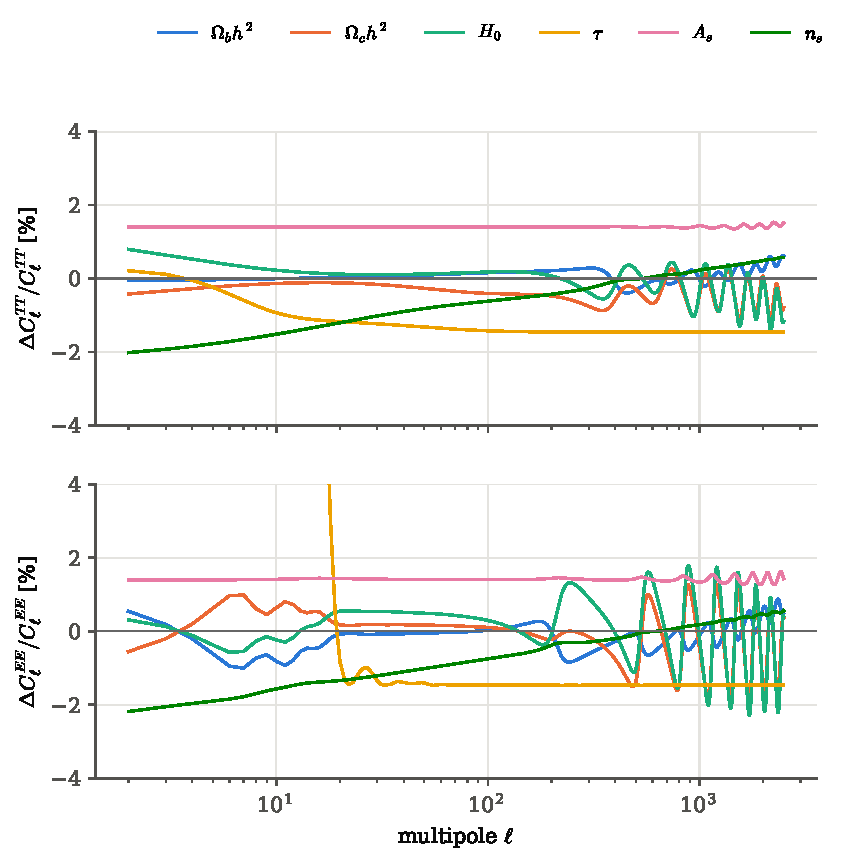
\includegraphics[width=0.86\linewidth]{figures/chT1/cl_response.pdf}
\caption{Fractional change of the lensed $TT$ (top) and $EE$ (bottom) spectra when each $\Lambda$CDM parameter moves by its Planck $1\sigma$ error, \cref{T1a:eq:response}. A flat line is a pure change of amplitude, a slanted line is a tilt, and a wiggle means the acoustic peaks change height or position. The $\tau$ curve in $EE$ leaves the plot at low $\ell$ (it reaches $\TOneTauRespEElow\%$).}
\label{T1a:fig:cl-response}
\end{figure}

\Cref{T1a:fig:cl-response} shows the six responses. Each can be read physically in one sentence:
\begin{itemize}[leftmargin=1.4em,itemsep=2pt]
\item $A_s$: a flat $+\TOneAsRespHigh\%$ at every $\ell$, because the primordial amplitude multiplies the whole spectrum.
\item $\tau$: a flat $\TOneTauRespHigh\%$ for $\ell\gtrsim30$, the $e^{-2\tau}$ screening of the anisotropies by the reionised electrons, with no effect on the largest scales of $TT$ and a large rise ($\TOneTauRespEElow\%$) in the low-$\ell$ $EE$ reionisation bump, which those same electrons create (see the cosmology notes).
\item $n_s$: a straight line in $\ln\ell$, rotating the spectrum about $\ell\approx\TOneNsPivotEll$, since a tilt adds power on one side of the pivot and removes it on the other.
\item $\Omega_{b0}h^2$ and $\Omega_{c0}h^2$: wiggles in phase with the acoustic peaks, largest $\TOneMaxRespOmc\%$ for $\Omega_{c0}h^2$, because the baryon loading and the epoch of matter--radiation equality set the relative heights of the peaks (see the cosmology notes).
\item $H_0$, at fixed physical densities: a slow drift at low $\ell$ from the late-time decay of the potentials, and oscillations at high $\ell$ because a changed distance to last scattering slides every peak sideways in $\ell$ (see the cosmology notes).
\end{itemize}

Two of these curves are nearly the same curve with opposite sign. Above $\ell\approx30$ the $A_s$ response is flat and positive, and the $\tau$ response is flat and negative. How alike are they? Treat each response as a list of numbers, one per $\ell$, and compute the cosine of the angle between the two lists, giving each $\ell$ the weight $2\ell+1$ (the number of $\alm$ at that $\ell$). A cosine of $+1$ or $-1$ means the same shape up to a factor. Over $30\le\ell\le\TOneLmax$ it is $\TOneCosAsTauTT$. The reason is visible in the list above: at high $\ell$ the spectrum is proportional to $A_s$ times the screening factor $e^{-2\tau}$, so it depends on the two only through $A_se^{-2\tau}$. Raise $A_s$ and raise $\tau$ together so that $A_se^{-2\tau}$ stays fixed, and the high-$\ell$ spectrum does not change. \Cref{T1a:fig:as-tau} puts $+R_{A_s}$ on top of $-R_\tau$ to make this visible.

\begin{figure}[htbp]
\centering
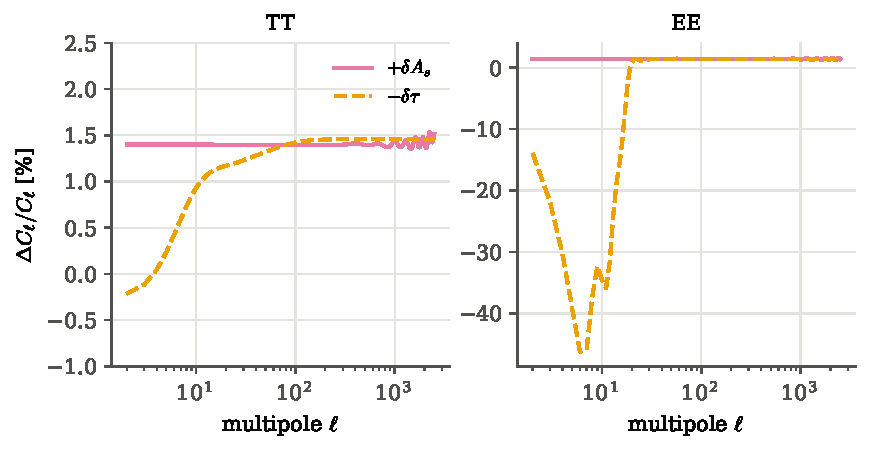
\includegraphics[width=0.9\linewidth]{figures/chT1/as_tau_degeneracy.pdf}
\caption{The $A_s$--$\tau$ degeneracy. The solid curve is the response to $+1\sigma$ in $A_s$, the dashed curve minus the response to $+1\sigma$ in $\tau$. In $TT$ (left) they coincide for $\ell\gtrsim30$, so high-$\ell$ temperature data measure only the combination $A_se^{-2\tau}$. In $EE$ (right) they separate completely at $\ell\lesssim20$, where the reionisation bump responds to $\tau$ alone.}
\label{T1a:fig:as-tau}
\end{figure}

This is what a degeneracy looks like before any statistics is done: two columns of derivatives that are almost parallel. In \cref{ch:10} it makes the Fisher matrix nearly singular along one direction. As a result, the marginalised errors on $A_s$ and $\tau$ (each parameter's error when the other is left free) are far larger than the conditional ones (its error when the other is held fixed). In \cref{ch:09} the same degeneracy appears as a long, thin ridge in the MCMC samples of $(\ln10^{10}A_s,\tau)$. The right panel shows how it is broken in practice. Large-angle polarisation measures $\tau$ on its own, and $A_s$ then follows from the high-$\ell$ amplitude.

\begin{inpractice}[Verification and research]
Here the finite differences only \emph{verify} what the physics already tells us (a flat $A_s$ response, the $e^{-2\tau}$ screening, the tilt about a pivot). In a Fisher forecast the same derivatives are the research instrument, and their accuracy has to be tested: the step must be small enough that $\Cell$ is linear in $\theta_i$ over $\pm\delta_i$, and large enough that CAMB's numerical noise does not dominate the difference. The standard check is to halve and double $\delta_i$ and confirm that the derivative does not move; \cref{ch:10} does this.
\end{inpractice}

\section{Experiment 2: the matter power spectrum and the BAO bump}
\label{T1a:sec:pk}

The second experiment turns to the matter field, the three-dimensional counterpart of the CMB sky. CAMB returns the matter power spectrum $P(k)$ at any redshift, either in linear theory or with the halofit correction \cite{Takahashi2012} \unpack{a fit to $N$-body simulations that maps the linear $P(k)$ to the non-linear one}. From the linear $P(k)$ we compute two things ourselves. The first is the correlation function $\xi(r)$, from the Fourier integral in the $P(k)$ row of the last table in \cref{T1a:sec:objects}. The second is $\sigma_8$, from the top-hat integral in the $\sigma_8$ row. CAMB also reports $\sigma_8$, so the second is a check on our code.

\pyfile[firstline=48,lastline=61,firstnumber=48]{code/chT1/02_pk_xi.py}{$\xi(r)$ and $\sigma_R$ from the linear $P(k)$}

\pyname{xi_of_r} evaluates $\xi(r)=\int\frac{\dd k}{2\pi^2}k^2P(k)\frac{\sin kr}{kr}$ as an integral over $\ln k$. Since $\dd k=k\,\dd\ln k$, the factor $k^2\,\dd k$ becomes $k^3\,\dd\ln k$; that is the $k^3$ in line 53. (\pyname{np.sinc(x/np.pi)} is $\sin x/x$.) The factor $e^{-k^2s^2}$ with $s=1\,h^{-1}$Mpc in line 51 is there only so the integral converges: it damps the fast-oscillating tail of the integrand. It acts on scales a hundred times smaller than the BAO peak and does not move the peak. \pyname{tophat_sigma} is the $\sigma_R$ integral with the window $W_R(k)=3(\sin kR-kR\cos kR)/(kR)^3=3j_1(kR)/(kR)$. At $R=8\,h^{-1}$Mpc it gives $\sigma_8=\TOneSigmaEightOurs$, against CAMB's $\TOneSigmaEight$, and $\TOneSigmaEightZone$ at $z=1$, where structure has had less time to grow.

\begin{figure}[htbp]
\centering
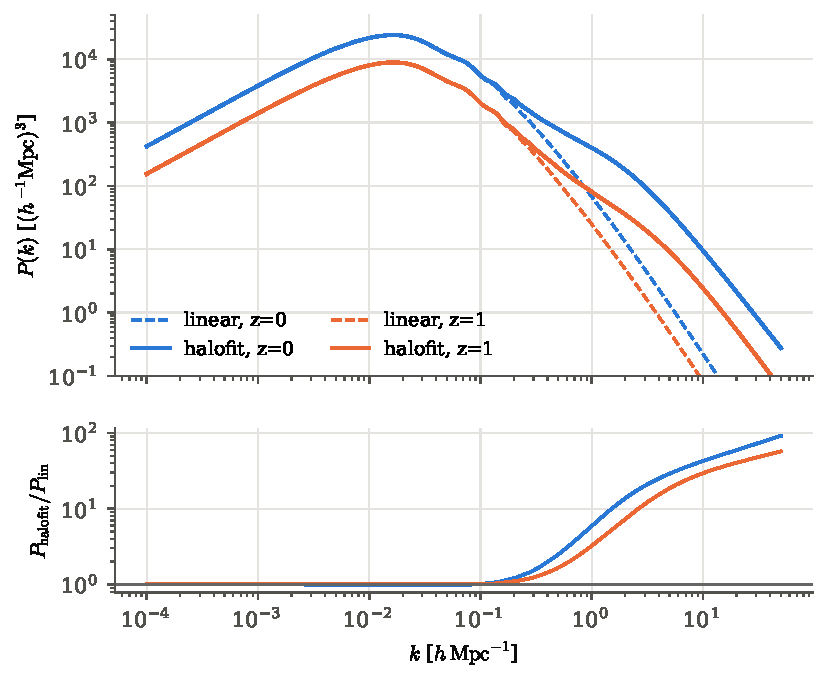
\includegraphics[width=0.8\linewidth]{figures/chT1/pk_lin_nl.pdf}
\caption{Matter power spectrum of the fiducial model at $z=0$ (blue) and $z=1$ (orange), linear theory dashed and halofit solid. The lower panel is the ratio halofit/linear: the two agree on large scales and differ by $10\%$ at $k\approx\TOneKnl\,h\,\mathrm{Mpc}^{-1}$ at $z=0$, and only at $k\approx\TOneKnlZone\,h\,\mathrm{Mpc}^{-1}$ at $z=1$.}
\label{T1a:fig:pk}
\end{figure}

\Cref{T1a:fig:pk} shows two pieces of physics.

The first is the turnover at $k\approx\TOneKpeak\,h\,\mathrm{Mpc}^{-1}$. It marks the size of the horizon at matter--radiation equality. Modes with larger $k$ (smaller scales) entered the horizon earlier, during radiation domination, and grew little there. So the transfer function falls roughly as $(k_{\mathrm{eq}}/k)^2$ (up to a logarithm), where $k_{\mathrm{eq}}$ is the turnover wavenumber. Since $P(k)\propto k^{n_s}T^2$ and $n_s\approx1$, beyond the turnover $P(k)$ falls roughly as $k\cdot k^{-4}=k^{-3}$ (see the cosmology notes).

The second is where halofit leaves linear theory. At $z=0$ the two differ by $10\%$ at $k\approx\TOneKnl\,h\,\mathrm{Mpc}^{-1}$ and by a factor $\TOneRatioOne$ at $k=1\,h\,\mathrm{Mpc}^{-1}$. The reason is gravitational collapse into haloes, which piles up power on small scales. For the statistics this boundary matters more than any number on the plot. On large scales the matter field is close to Gaussian, and $P(k)$ carries all of its information; this is the regime of the Gaussian random fields of \cref{ch:07}. On small scales the field is non-Gaussian, and $P(k)$ no longer tells the whole story. There, summaries that see the shape of the field, the topological summaries of \cref{ch:12}, have something extra to find.

\begin{figure}[htbp]
\centering
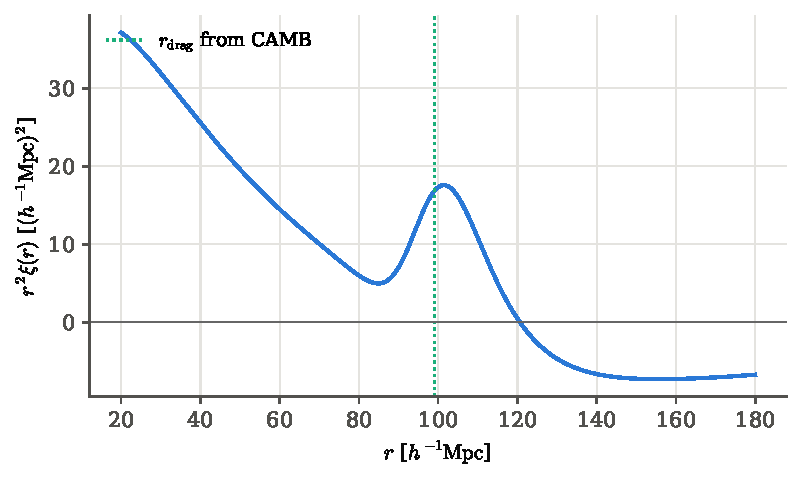
\includegraphics[width=0.8\linewidth]{figures/chT1/xi_bao.pdf}
\caption{The linear correlation function at $z=0$, multiplied by $r^2$ so that the bump is visible. The peak at $r\approx\TOneRpeak\,h^{-1}$Mpc sits close to the drag-epoch sound horizon computed by CAMB (dotted line, $\TOneRdragH\,h^{-1}$Mpc).}
\label{T1a:fig:xi}
\end{figure}

\Cref{T1a:fig:xi} shows the same information in real space, and there the baryon acoustic oscillations are much easier to see. In $P(k)$ they are small wiggles on a steep curve. In $\xi(r)$ they collapse into a single bump near $r\approx\TOneRpeak\,h^{-1}$Mpc. Where does the bump come from? Each initial overdensity launched a spherical sound wave into the photon--baryon plasma. The wave travelled until the baryons were released from the photons at the drag epoch, and then stopped. Its radius at that moment is the sound horizon $r_s(z_{\mathrm{drag}})$ of the BAO row, and it leaves an excess of pairs of points at that separation (see the cosmology notes). CAMB gives $r_s(z_{\mathrm{drag}})=\TOneRdrag$\,Mpc, that is $\TOneRdragH\,h^{-1}$Mpc. The peak of $r^2\xi$ sits a couple of percent higher because it rides on the sloping broad-band part of $\xi$.

Why does this matter? The CMB fixes $r_s$ precisely, so the bump is a ruler of known length. Its observed position in a galaxy survey at redshift $z$ therefore measures $D_A(z)$ (from its angular size) and $H(z)$ (from its extent along the line of sight). This is how BAO data enter the parameter fits mentioned in \cref{ch:05}. The bump was first detected in the galaxy correlation function by \cite{Eisenstein2005}. In \cref{ch:07} it is a feature to recover from a simulated field with noisy estimates of $\xi(r)$. In \cref{ch:12} it is one of the structures that a summary beyond the two-point function must respect.

\begin{recap}
\begin{itemize}[leftmargin=1.2em,itemsep=1pt]
\item Six numbers $(\Omega_{b0}h^2,\Omega_{c0}h^2,H_0\text{ or }\theta_{\mathrm{MC}},\tau,A_s,n_s)$ go into CAMB; out come $E(z)$ and distances, $\Cell$, $P(k)$, $\xi(r)$, $\sigma_8$.
\item The model predicts statistics, $\Cell=\langle\abs{\alm}^2\rangle$ and $P(k)$, never the $\alm$ or $\delta_{\bm k}$ themselves. Our sky is one draw.
\item Conventions: raw $\Cell$ (not $D_\ell$) in all statistics; $\mu\mathrm K^2$ means a factor $T_0^2$; CAMB's $A_s=\frac{25}{4}A_S^2$ of the cosmology notes; $P(k)$ in $(h^{-1}\mathrm{Mpc})^3$; CAMB's $\phi$ is the notes' $\psi$.
\item Nudging each parameter by $1\sigma$ gives $\partial\Cell/\partial\theta_i$, the Fisher derivatives; $A_s$ and $\tau$ respond identically above $\ell\approx30$ (cosine $\TOneCosAsTauTT$), and low-$\ell$ $EE$ breaks the tie.
\item Linear and halofit $P(k)$ separate at $k\approx\TOneKnl\,h\,\mathrm{Mpc}^{-1}$ today; $\xi(r)$ has the BAO bump near $r_s(z_{\mathrm{drag}})\approx\TOneRdragH\,h^{-1}$Mpc; our $\sigma_8$ matches CAMB's to better than $0.1\%$.
\end{itemize}
\end{recap}

\providecommand{\TOneSigmaEight}{}\renewcommand{\TOneSigmaEight}{0.8111}
\providecommand{\TOneSigmaEightOurs}{}\renewcommand{\TOneSigmaEightOurs}{0.8112}
\providecommand{\TOneSigmaEightZone}{}\renewcommand{\TOneSigmaEightZone}{0.4928}
\providecommand{\TOneRdrag}{}\renewcommand{\TOneRdrag}{147.10}
\providecommand{\TOneRdragH}{}\renewcommand{\TOneRdragH}{99.1}
\providecommand{\TOneRpeak}{}\renewcommand{\TOneRpeak}{101.5}
\providecommand{\TOneKnl}{}\renewcommand{\TOneKnl}{0.15}
\providecommand{\TOneKnlZone}{}\renewcommand{\TOneKnlZone}{0.21}
\providecommand{\TOneKpeak}{}\renewcommand{\TOneKpeak}{0.017}
\providecommand{\TOneRatioOne}{}\renewcommand{\TOneRatioOne}{5.9}
\providecommand{\TOneSEightFid}{}\renewcommand{\TOneSEightFid}{0.832}
\providecommand{\TOneZmed}{}\renewcommand{\TOneZmed}{0.71}
\providecommand{\TOneZmedLo}{}\renewcommand{\TOneZmedLo}{0.49}
\providecommand{\TOneZmedHi}{}\renewcommand{\TOneZmedHi}{0.99}
\providecommand{\TOneSigEightLo}{}\renewcommand{\TOneSigEightLo}{0.911}
\providecommand{\TOneSigEightHi}{}\renewcommand{\TOneSigEightHi}{0.720}
\providecommand{\TOneAlongMax}{}\renewcommand{\TOneAlongMax}{9}
\providecommand{\TOneAlongMedLo}{}\renewcommand{\TOneAlongMedLo}{-4}
\providecommand{\TOneAlongMedHi}{}\renewcommand{\TOneAlongMedHi}{+7}
\providecommand{\TOneAcrossLo}{}\renewcommand{\TOneAcrossLo}{-22}
\providecommand{\TOneAcrossHi}{}\renewcommand{\TOneAcrossHi}{+24}
\providecommand{\TOneLimberErr}{}\renewcommand{\TOneLimberErr}{0.1}
\providecommand{\TOneDlnCdlnSEight}{}\renewcommand{\TOneDlnCdlnSEight}{2.8}
\providecommand{\TOneDlnCdlnOm}{}\renewcommand{\TOneDlnCdlnOm}{1.6}
\providecommand{\TOneAlphaGalTwo}{}\renewcommand{\TOneAlphaGalTwo}{0.59}
\providecommand{\TOneAlphaGalTwoK}{}\renewcommand{\TOneAlphaGalTwoK}{0.62}
\providecommand{\TOneAlphaLoFive}{}\renewcommand{\TOneAlphaLoFive}{0.58}
\providecommand{\TOneAlphaFive}{}\renewcommand{\TOneAlphaFive}{0.55}
\providecommand{\TOneAlphaHiFive}{}\renewcommand{\TOneAlphaHiFive}{0.53}
\providecommand{\TOneNoiseOne}{}\renewcommand{\TOneNoiseOne}{4.965\times10^{-9}}
\providecommand{\TOneFsky}{}\renewcommand{\TOneFsky}{0.0242}
\providecommand{\TOneEdgeOne}{}\renewcommand{\TOneEdgeOne}{0.43}
\providecommand{\TOneEdgeFour}{}\renewcommand{\TOneEdgeFour}{1.05}
\providecommand{\TOneLeqOne}{}\renewcommand{\TOneLeqOne}{21}
\providecommand{\TOneLeqThree}{}\renewcommand{\TOneLeqThree}{87}
\providecommand{\TOneLeqFive}{}\renewcommand{\TOneLeqFive}{194}
\providecommand{\TOneSNtomo}{}\renewcommand{\TOneSNtomo}{48}
\providecommand{\TOneSNone}{}\renewcommand{\TOneSNone}{42}
\providecommand{\TOneSigLnSEight}{}\renewcommand{\TOneSigLnSEight}{0.8}
\providecommand{\TOneLmaxSN}{}\renewcommand{\TOneLmaxSN}{2000}
\providecommand{\TOneSigmaE}{}\renewcommand{\TOneSigmaE}{0.27}
\providecommand{\TOneNeff}{}\renewcommand{\TOneNeff}{6.2}
\providecommand{\TOneArea}{}\renewcommand{\TOneArea}{1000}
 
\section{Weak lensing: the matter field written on galaxy shapes}
\label{T1b:sec:shapes}

Light from a distant galaxy crosses billions of light years of clumpy matter on its way to us. Every lump it passes bends it a little. What arrives is an image that is slightly displaced, slightly enlarged and slightly stretched in one direction, typically by about one per cent. Nothing in the image says which part of it is the stretch: a galaxy that looks elongated may simply be elongated. Yet the stretch is the cleanest probe of matter we have, because gravity bends light whatever the matter is made of, dark or luminous, and no assumption about how galaxies trace mass enters. This is \newterm{weak gravitational lensing}, and \newterm{cosmic shear} is its version with the large-scale structure as the lens \cite{BartelmannSchneider2001,Kilbinger2015}.

For the data analyst, weak lensing is the situation of \cref{T1a:sec:machine} in a sharper form. There the model predicted the variance $\Cell$ of the CMB sky and the sky was one draw. Here the model predicts the angular power spectrum $C_\ell^{\kappa\kappa}$ of a lensing field $\kappa$ (defined below), the sky gives one draw of $\kappa$, and on top of that we do not see $\kappa$ itself. We see the shapes of galaxies, and each shape is mostly the galaxy's own.

\paragraph{The question.}
What we observe is a catalogue: for every galaxy, a position on the sky and an \newterm{ellipticity} \unpack{a complex number $\varepsilon=\varepsilon_1+i\varepsilon_2$ whose size is how elongated the image is and whose phase is twice the angle of its long axis}. What could have produced the ellipticity of one particular galaxy? There are two candidates, and we take them one at a time.
\begin{enumerate}[leftmargin=1.6em,itemsep=2pt]
\item \emph{The galaxy's own shape.} Galaxies are not round. Their intrinsic ellipticities $\varepsilon^{(0)}$ scatter with an rms $\sigma_e\approx0.27$ per component \cite{Asgari2021KiDS}, and their long axes point in random directions. So the intrinsic part has mean zero, but it is large.
\item \emph{The shear of the matter in front of it.} The lensing stretch $\gamma$ is about $0.01$, thirty times smaller. But it is \emph{coherent}: two galaxies that lie close together on the sky sent their light past the same lumps, so they are stretched in nearly the same way.
\end{enumerate}
Only now do we compute anything. In the weak regime the two simply add,
\begin{equation}
\varepsilon\approx\varepsilon^{(0)}+\gamma .
\label{T1b:eq:eps-sum}
\end{equation}
The reason is that $\varepsilon$ is defined from the shape of the image, and a shear of one per cent changes that shape by one per cent: to first order in small quantities it moves the ellipticity by $\gamma$ itself, whatever the galaxy's own shape was. \Cref{T1b:sec:reduced-shear} works this out for a round source; with the other common definition of $\varepsilon$ the shift is $2\gamma$ instead (convention~3 of \cref{T1b:sec:conventions}). A single galaxy tells us almost nothing, since the shear is buried under a noise thirty times larger. But the intrinsic parts of different galaxies are independent, and the shears of neighbours are correlated. Two moves turn this into a measurement.

\emph{Average galaxies that share one shear.} Take $N$ galaxies close enough together that they all feel the same $\gamma$, and average their ellipticities:
\begin{align}
\bar\varepsilon\equiv\frac1N\sum_{a=1}^N\varepsilon_a
&\eqby{1}\gamma+\frac1N\sum_{a=1}^N\varepsilon^{(0)}_a,
&
\E\,\bar\varepsilon&\eqby{2}\gamma,
&
\Var\bar\varepsilon_1&\eqby{3}\frac{\sigma_e^2}{N}.
\label{T1b:eq:shear-mean}
\end{align}
\begin{explain}
  \item Insert \eqref{T1b:eq:eps-sum} for each galaxy; the shear is the same in every term, so its average is itself.
  \item The intrinsic ellipticities point in random directions, so each has mean zero.
  \item The variance of a mean of $N$ independent readings of variance $\sigma_e^2$, \eqref{3a:eq:var-mean}, applied to one real component; the same holds for $\bar\varepsilon_2$.
\end{explain}
So the noise on the shear estimate is $0.27/\sqrt N$ per component. How large must $N$ be? A signal-to-noise ratio of one on a single shear of $0.01$ needs $0.27/\sqrt N=0.01$, that is $N=(0.27/0.01)^2\approx730$ galaxies, all sharing that one shear. A map with many independent shear values, each measured several times better than that, needs millions of galaxies.

\emph{Correlate pairs.} The shear changes across the sky, so averaging is limited to small patches. Correlation uses every pair instead. For two galaxies $a\neq b$, multiply the ellipticity of one by the complex conjugate of the other and expand:
\begin{align}
\bigl\langle\varepsilon_a\varepsilon_b^*\bigr\rangle
&\eqby{1}\bigl\langle(\varepsilon^{(0)}_a+\gamma_a)(\varepsilon^{(0)}_b+\gamma_b)^*\bigr\rangle\nonumber\\
&\eqby{2}\bigl\langle\varepsilon^{(0)}_a\varepsilon^{(0)*}_b\bigr\rangle+\bigl\langle\varepsilon^{(0)}_a\gamma_b^*\bigr\rangle+\bigl\langle\gamma_a\varepsilon^{(0)*}_b\bigr\rangle+\bigl\langle\gamma_a\gamma_b^*\bigr\rangle
\eqby{3}\bigl\langle\gamma_a\gamma_b^*\bigr\rangle .
\label{T1b:eq:pair}
\end{align}
\begin{explain}
  \item \Cref{T1b:eq:eps-sum} for each galaxy.
  \item Multiply out the brackets; the average of a sum is the sum of the averages.
  \item The intrinsic shapes of two different galaxies are independent, each with mean zero, so the first term is the product of two zero means. In the two middle terms an intrinsic shape is independent of the shear in front of the other galaxy, and the same reasoning makes them vanish. Only the correlation of the shears survives.
\end{explain}
Galaxy $a$ paired with itself would add $\langle\abs{\varepsilon^{(0)}_a}^2\rangle$, which does not vanish; this is why the self-pairs are left out, and why shape noise reappears as an added term in the power spectrum (\cref{T1b:sec:objects}). The information is in the statistics of many shapes, never in one shape. This is why every weak-lensing number in the later chapters is a two-point function, a peak count or a topological summary of a field built from millions of galaxies, and why its noise term is set by how many galaxies there are.

\Cref{T1b:fig:kappa-gamma} shows what the two parts of the lensing distortion do, exaggerated twenty-five-fold. The \newterm{convergence} $\kappa$ \unpack{the projected matter density along the line of sight, in units of a critical density} enlarges an image without changing its shape. The \newterm{shear} $\gamma=\gamma_1+i\gamma_2$ \unpack{the tidal part of the lensing distortion, which stretches the image along one axis and squeezes it along the perpendicular one} turns a circle into an ellipse.

\begin{figure}[htbp]
\centering
\begin{tikzpicture}[scale=1.0]
  \def\r{0.6}
  \draw[thick,formblue] (0,0) circle (\r);
  \node[font=\small] at (0,-1.35) {source};
  \draw[thick,formblue] (2.4,0) circle ({\r/(1-0.25)});
  \node[font=\small] at (2.4,-1.35) {$\kappa=0.25$ only};
  \draw[thick,formblue] (4.9,0) ellipse ({\r/(1-0.25)} and {\r/(1+0.25)});
  \node[font=\small] at (4.9,-1.35) {$\gamma_1=0.25$ only};
  \draw[softgray,dashed] (2.4,0) circle (\r);
  \draw[softgray,dashed] (4.9,0) circle (\r);
  \node[font=\small\bfseries] at (-0.9,1.15) {(a)};
  \begin{scope}[xshift=8.0cm]
    \node[font=\small\bfseries] at (-1.3,1.15) {(b)};
    \fill[bdryred] (0,0) circle (0.08);
    \foreach \t in {0,30,...,330} {
      \draw[very thick,tangentgreen] ({0.85*cos(\t)+0.15*cos(\t+90)},{0.85*sin(\t)+0.15*sin(\t+90)})
        -- ({0.85*cos(\t)-0.15*cos(\t+90)},{0.85*sin(\t)-0.15*sin(\t+90)});
    }
    \node[font=\small,align=center] at (0,-1.35) {$E$ mode};
  \end{scope}
  \begin{scope}[xshift=11.0cm]
    \fill[bdryred] (0,0) circle (0.08);
    \foreach \t in {0,30,...,330} {
      \draw[very thick,fibreorange] ({0.85*cos(\t)+0.15*cos(\t+45)},{0.85*sin(\t)+0.15*sin(\t+45)})
        -- ({0.85*cos(\t)-0.15*cos(\t+45)},{0.85*sin(\t)-0.15*sin(\t+45)});
    }
    \node[font=\small,align=center] at (0,-1.35) {$B$ mode};
  \end{scope}
\end{tikzpicture}
\caption{(a) A round source (left), the same source magnified by convergence alone (middle), and stretched by shear alone (right); the dashed circle is the source for comparison. Real values are near $0.01$, not $0.25$. (b) Each stick is the long axis of a sheared image. Around a mass concentration (red dot) lensing lines the images up tangentially, the $E$ pattern. Rotating every stick by $45^\circ$ gives the $B$ pattern, a swirl, which lensing by a scalar potential cannot make.}
\label{T1b:fig:kappa-gamma}
\end{figure}

The sticks in panel (b) have no arrowheads, and that is the key property of shear. An ellipse rotated by $180^\circ$ is the same ellipse. What kind of number can describe such a stick?

\emph{A stick first.} Let the long axis of an ellipse make an angle $\phi$ with the first reference axis. If we turn the reference axes by an angle $\alpha$, the same stick is now seen at $\phi-\alpha$. A complex number that records the direction must be a function $f(\phi)$, and the simplest functions of an angle are the pure tones $e^{im\phi}$ with a whole number $m$. Which $m$ will do? The stick at $\phi+\pi$ is the same stick, so we need $e^{im(\phi+\pi)}=e^{im\phi}$, that is $e^{im\pi}=1$, and $m$ must be even. The choice $m=1$ fails: $e^{i(\phi+\pi)}=-e^{i\phi}$, so the same stick would get two opposite values. That is the description of an arrow, a vector, which returns to itself only after a full turn of $2\pi$. The choice $m=0$ is allowed but records no direction at all. The smallest useful choice is $m=2$, so a stretch of size $\abs\gamma$ along the angle $\phi$ is written $\gamma=\abs\gamma e^{2i\phi}$, the form in the table of \cref{T1b:sec:objects}. When the axes turn by $\alpha$,
\begin{equation}
\gamma=\abs\gamma e^{2i\phi}\ \longrightarrow\ \abs\gamma e^{2i(\phi-\alpha)}=e^{-2i\alpha}\gamma .
\label{T1b:eq:spin2}
\end{equation}
A quantity that picks up the phase $e^{-is\alpha}$ under a turn of the axes is said to have \newterm{spin} $s$. Shear has spin 2. The CMB polarization $Q+iU$ is also a headless stick and changes in exactly the same way (see the cosmology notes). Every tool built for CMB polarization (the split into $E$ and $B$ modes, spin-2 spherical harmonics, \pyname{healpy}'s polarization transforms) uses only the rule \eqref{T1b:eq:spin2}, so it applies to shear without change.

\emph{Where the two angles live.} Every lensing formula below is written in two angles, $\theta_1$ and $\theta_2$. They locate a point on the sky the way $x$ and $y$ locate a point on a sheet of graph paper held at arm's length. The patch we analyse is a few degrees across at most, so we may treat it as flat: a plane facing us, with its origin on one chosen line of sight (in \cref{T1b:fig:sky-plane}, the one through a lump of matter), and $\theta_1$, $\theta_2$ the two angles, measured from that line, to a point on it. Now follow the light of one galaxy. Without the lump, the galaxy would be seen in the direction $\bm\theta_S$ where it really is. The light that actually reaches us left the galaxy in a slightly different direction, was bent as it passed the lump, and arrives along a straight final leg. We place every object where its light appears to come from, so we extend that last leg backwards, and it meets the sky plane at a different point, $\bm\theta$. The catalogue records $\bm\theta$; the true $\bm\theta_S$ is never seen. The difference is the deflection, $\bm\theta_S=\bm\theta-\hat{\bm\alpha}(\bm\theta)$, the second row of the table in \cref{T1b:sec:objects}.

The deflection by itself changes nothing we can measure. If every point of a galaxy moved by the same $\hat{\bm\alpha}$, the image would simply be the galaxy, displaced, and we never know where it would have been. What we can measure is how the deflection \emph{changes} across one image: points on the side nearer the lump are pulled more than points on the far side, so the image is enlarged ($\kappa$) and stretched ($\gamma$). Panel (b) of \cref{T1b:fig:sky-plane} shows the outcome for the lump of the figure: the image is pushed outward and stretched along the circle around the lump, the tangential pattern of \cref{T1b:fig:kappa-gamma}(b).

\begin{figure}[htbp]
\centering
\begin{tikzpicture}[scale=0.84,>={Stealth[length=2.2mm]}]
  \def\ux{0.9}\def\uy{0.5}
  \node[font=\small\bfseries] at (-0.6,3.3) {(a)};
  \fill (0,0) circle (0.09);
  \node[font=\small,below=2pt] at (0,0) {us};
  \coordinate (Lc) at (5,0);
  \draw[softgray!70,fill=softgray!8]
    ($(Lc)+(-1.0*\ux,-1.0*\uy)+(0,-1.3)$) -- ($(Lc)+(1.0*\ux,1.0*\uy)+(0,-1.3)$) --
    ($(Lc)+(1.0*\ux,1.0*\uy)+(0,1.7)$) -- ($(Lc)+(-1.0*\ux,-1.0*\uy)+(0,1.7)$) -- cycle;
  \shade[ball color=bdryred!80] (Lc) circle (0.17);
  \node[font=\small,softgray,below] at ($(Lc)+(0,-1.85)$) {lump of matter};
  \coordinate (Sc) at (10,0);
  \draw[formblue!70,fill=formblue!5]
    ($(Sc)+(-2.2*\ux,-2.2*\uy)+(0,-1.4)$) -- ($(Sc)+(2.2*\ux,2.2*\uy)+(0,-1.4)$) --
    ($(Sc)+(2.2*\ux,2.2*\uy)+(0,2.9)$) -- ($(Sc)+(-2.2*\ux,-2.2*\uy)+(0,2.9)$) -- cycle;
  \node[font=\small,formblue,below] at ($(Sc)+(0,-2.6)$) {sky plane};
  \draw[->,thick] ($(Sc)+(-1.6*\ux,-1.6*\uy)$) -- ($(Sc)+(2.0*\ux,2.0*\uy)$) node[below right=-1pt,font=\small] {$\theta_1$};
  \draw[->,thick] ($(Sc)+(0,-1.2)$) -- ($(Sc)+(0,2.7)$) node[above,font=\small] {$\theta_2$};
  \draw[softgray,dashed] (0,0) -- (Sc);
  \coordinate (S) at ($(Sc)+(0.4*\ux,0.4*\uy)+(0,0.5)$);
  \coordinate (P) at ($(Sc)+(1.0*\ux,1.0*\uy)+(0,1.25)$);
  \coordinate (L) at ($(0,0)!0.5!(P)$);
  \draw[dotted,thick] (P) -- ($(Sc)+(1.0*\ux,1.0*\uy)$);
  \draw[dotted,thick] (P) -- ($(Sc)+(0,1.25)$);
  \draw[very thick,tangentgreen,postaction={decorate},
        decoration={markings,mark=at position 0.55 with {\arrow{<}}}] (L) -- (S);
  \draw[very thick,tangentgreen,postaction={decorate},
        decoration={markings,mark=at position 0.45 with {\arrow{<}}}] (0,0) -- (L);
  \draw[thick,fibreorange,dashed] (L) -- (P);
  \draw[->,thick,black] ($(S)!0.17!(P)$) -- ($(S)!0.83!(P)$);
  \draw[thick,tangentgreen,fill=white] (S) circle (0.1);
  \fill[fibreorange] (P) circle (0.1);
  \draw[tangentgreen,thin] (S) -- ($(S)+(0.5,-1.15)$) node[below,font=\small] {$\bm\theta_S$, true};
  \node[font=\small,fibreorange,above right=1pt] at (P) {$\bm\theta$, seen};
  \node[font=\small,right=1pt] at ($(S)!0.55!(P)$) {$\hat{\bm\alpha}$};
  \begin{scope}[xshift=15.4cm,yshift=0.45cm]
    \node[font=\small\bfseries] at (-2.6,2.55) {(b)};
    \fill[formblue!5] (-2.2,-2.2) rectangle (2.2,2.2);
    \draw[formblue!18,very thin,step=0.4] (-2.2,-2.2) grid (2.2,2.2);
    \draw[formblue!70] (-2.2,-2.2) rectangle (2.2,2.2);
    \node[font=\small,formblue,below] at (0,-2.25) {sky plane, face on};
    \draw[->,thick] (-2.0,0) -- (2.0,0) node[below=1pt,font=\small] {$\theta_1$};
    \draw[->,thick] (0,-2.0) -- (0,2.0) node[left=1pt,font=\small] {$\theta_2$};
    \draw[softgray] (0,0) circle (1.6);
    \shade[ball color=bdryred!80] (0,0) circle (0.13);
    \draw[dotted,thick] (1.28,1.6) -- (1.28,0);
    \draw[dotted,thick] (1.28,1.6) -- (0,1.6);
    \draw[thick,tangentgreen,dashed,fill=white] (0.512,0.64) circle (0.22);
    \draw[->,thick] (0.66,0.83) -- (1.1,1.38);
    \draw[thick,fibreorange,fill=fibreorange!30,rotate around={-38.66:(1.28,1.6)}] (1.28,1.6) ellipse (0.38 and 0.17);
  \end{scope}
\end{tikzpicture}
\caption{What the two angles $\theta_1,\theta_2$ are. (a) A patch of sky, treated as a flat plane facing us, with its origin on the line of sight through a lump of matter (dashed grey). A galaxy sits at the true position $\bm\theta_S$ (open green circle). Its light (solid green) is bent where it passes the lump, so it reaches us along a final leg that, extended backwards (dashed orange), meets the sky plane at $\bm\theta$ (orange dot): this is where the galaxy is seen and catalogued, and the dotted lines read off its two coordinates. The black arrow, from the true position to the seen one, is the deflection $\hat{\bm\alpha}=\bm\theta-\bm\theta_S$. (b) The same patch face on. The round galaxy (dashed green) is seen further from the lump and stretched along the grey circle around it, tangentially. The deflection is exaggerated enormously; the lens drawn halfway is for clarity, any lump between us and the galaxy acts the same way.}
\label{T1b:fig:sky-plane}
\end{figure}

\emph{The pattern around a lump.} Does the formula of the table, $\gamma_1=\frac12(\psi_{,11}-\psi_{,22})$, $\gamma_2=\psi_{,12}$, really give the tangential sticks of panel (b)? Take the simplest lens, a point mass at the origin, whose potential on the sky is $\psi=A\ln\theta$ with $A>0$ and $\theta=\sqrt{\theta_1^2+\theta_2^2}$. On the first axis, at $(\theta_1,0)$ with $\theta_1>0$,
\begin{align}
\psi_{,11}&\eqby{1}A\,\frac{\theta_2^2-\theta_1^2}{\theta^4}=-\frac{A}{\theta_1^2},
&
\psi_{,22}&\eqby{1}A\,\frac{\theta_1^2-\theta_2^2}{\theta^4}=+\frac{A}{\theta_1^2},
&
\psi_{,12}&\eqby{1}-\frac{2A\theta_1\theta_2}{\theta^4}=0,
\nonumber\\
\gamma_1&\eqby{2}-\frac{A}{\theta_1^2}<0,
&
\gamma_2&\eqby{2}0 .
\label{T1b:eq:point-shear}
\end{align}
\begin{explain}
  \item Differentiate $A\ln\theta=\frac A2\ln(\theta_1^2+\theta_2^2)$ twice, then set $\theta_2=0$.
  \item The shear components of the table.
\end{explain}
In panel (a) a positive $\gamma_1$ stretches the circle along the first axis, so a negative $\gamma_1$ stretches it along the second: on the first axis the stick stands vertical, at right angles to the line to the mass, which is tangential. Every other point follows from the rule \eqref{T1b:eq:spin2}: turning the axes so that the first one points at the new position leaves the same calculation. In complex form the result is $\gamma=-(A/\theta^2)e^{2i\varphi}=(A/\theta^2)e^{2i(\varphi+\pi/2)}$ at polar angle $\varphi$, a stick at angle $\varphi+90^\circ$, always tangential.

\emph{Why lensing makes no $B$.} The $E$ and $B$ rows of the second table of \cref{T1b:sec:objects} ($\Delta=\nabla^2$ is the angular Laplacian) split a shear field into the part whose sticks line up tangentially or radially about each point (rotation $0$) and the part whose sticks sit at $45^\circ$ (the swirl). Insert the lensing shear into the $B$ row:
\begin{align}
\Delta B
&\eqby{1}-2\partial_1\partial_2\,\tfrac12(\psi_{,11}-\psi_{,22})+(\partial_1^2-\partial_2^2)\,\psi_{,12}
\eqby{2}-\psi_{,1112}+\psi_{,1222}+\psi_{,1112}-\psi_{,1222}
=0,\nonumber\\
\Delta E
&\eqby{3}\tfrac12(\psi_{,1111}-2\psi_{,1122}+\psi_{,2222})+2\psi_{,1122}
=\tfrac12\Delta(\psi_{,11}+\psi_{,22})
\eqby{4}\Delta\kappa .
\label{T1b:eq:no-b}
\end{align}
\begin{explain}
  \item The $B$ row of the table with $\gamma_1=\frac12(\psi_{,11}-\psi_{,22})$ and $\gamma_2=\psi_{,12}$.
  \item Partial derivatives can be taken in any order, so the four fourth derivatives cancel in pairs.
  \item The $E$ row with the same substitution, multiplied out.
  \item $\kappa=\frac12\nabla^2\psi$, from the first table.
\end{explain}
A $B$ pattern needs a curl, and a shear built from the second derivatives of one scalar potential has none: lensing makes only $E$, and its $E$ is $\kappa$. A $B$ mode in the data therefore measures what went wrong, not what the cosmos did: residual errors in the correction for the telescope's point-spread function, intrinsic alignments, or approximations in the theory, and the astrophysical ones among these are at the per-cent level of the $E$ signal \cite[§3.6]{Kilbinger2015}, so a larger $B$ points to an error in the processing. Measuring $B$ and finding it consistent with zero is the standard \emph{null test} of a weak-lensing analysis, the lensing counterpart of the hypothesis tests of \cref{ch:04}.

\section{The objects a weak-lensing analysis uses}
\label{T1b:sec:objects}

A weak-lensing analysis is a chain of objects, each defined from the one before (\cref{T1b:fig:pipeline}). Light from a distant galaxy crosses the matter between us and it, and the matter bends the ray. That bending is described first at one point of the sky, by a single scalar potential and its derivatives. Next the three-dimensional matter field is projected along the line of sight, which gives the statistics of the sky that a model predicts. Last come the galaxy shapes, the noise they carry and the nuisances that stand between them and the model. For each object the question comes first, then the equation it starts from and the working equation of the book, then a size and the chapters that use it. The physics between the two equations is in the cosmology notes.

\begin{figure}[htbp]
\centering
\begin{tikzpicture}[
  box/.style={draw=accent,rounded corners=2pt,fill=ideabg,align=center,font=\small,
              minimum width=2.15cm,minimum height=1.05cm,inner sep=2pt,text width=2.1cm},
  nui/.style={draw=bdryred,rounded corners=2pt,fill=warnbg,align=center,font=\scriptsize,
              minimum width=2.15cm,minimum height=0.85cm,inner sep=2pt,text width=2.1cm},
  arr/.style={->,thick,accent}]
  \node[box] (d)  at (0,0)     {matter field\\ $\delta$, $P_\delta(k,z)$};
  \node[box] (k)  at (2.55,0)  {convergence\\ $\kappa(\bm\theta)$};
  \node[box] (g)  at (5.1,0)   {shear\\ $\gamma(\bm\theta)$};
  \node[box] (e)  at (7.65,0)  {ellipticities\\ $\varepsilon=\varepsilon^{(0)}+\gamma$};
  \node[box,fill=takebg,draw=tangentgreen] (s) at (10.2,0) {summary\\ $\widehat C_\ell^{\,ij}$, $\xi_\pm$, peaks};
  \draw[arr] (d) -- (k);
  \draw[arr] (k) -- (g);
  \draw[arr] (g) -- (e);
  \draw[arr] (e) -- (s);
  \node[nui] (b)  at (0,-1.75)    {baryonic feedback\\ alters $P_\delta$};
  \node[nui] (pz) at (2.55,-1.75) {photo-$z$ bins\\ set $p^{(i)}(z)$};
  \node[nui] (sb) at (5.1,-1.75)  {PSF, shear bias $m$\\ rescale $\gamma$};
  \node[nui] (ia) at (7.65,-1.75) {intrinsic alignment\\ correlates $\varepsilon^{(0)}$};
  \node[nui] (sn) at (10.2,-1.75) {shape noise\\ $\sigma_e^2/\bar n_i$};
  \draw[arr,bdryred] (b) -- (d);
  \draw[arr,bdryred] (pz) -- (k);
  \draw[arr,bdryred] (sb) -- (g);
  \draw[arr,bdryred] (ia) -- (e);
  \draw[arr,bdryred] (sn) -- (s);
\end{tikzpicture}
\caption{The weak-lensing chain. The matter field is projected into a convergence map, whose tidal part is the shear, which is added to the intrinsic shapes of the galaxies; the summary statistics are computed from those shapes. Each red box is a nuisance or noise source that enters at the object above it and has to be modelled and marginalised, or, for shape noise, added to the covariance.}
\label{T1b:fig:pipeline}
\end{figure}

\paragraph{The lens map at one point.}
The question is how the image of a source moves and deforms when matter lies in front of it. Work on a small patch of sky, treated as flat. The observed direction is $\bm\theta=(\theta_1,\theta_2)$, and $\bm\theta_S$ is the direction the source would have without lensing (\cref{T1b:fig:sky-plane}). A weak gravitational field perturbs the metric by the Newtonian potential $\Phi$ (equal to the second potential $\Psi$ when anisotropic stress is negligible), and a light ray in it is bent at each point by the transverse gradient of $\Phi$. Adding up the bends along the line of sight, each weighted by the geometry of the line of sight, gives one scalar, the \newterm{lensing potential}:
\begin{equation*}
\psi(\bm\theta,\chi)=\frac{2}{c^2}\int_0^\chi\!\dd\chi'\,\frac{f_K(\chi-\chi')}{f_K(\chi)f_K(\chi')}\,\Phi\bigl[f_K(\chi')\bm\theta,\chi'\bigr].
\end{equation*}
Here $\chi$ is comoving distance and $f_K(\chi)$ the curvature function ($f_K=\chi$ in a flat universe). Every lensing quantity is a derivative of $\psi$. The first derivative is the deflection, and it maps the observed position back to the true one:
\begin{equation*}
\hat{\bm\alpha}=\bm\nabla\psi,\qquad\bm\theta_S=\bm\theta-\bm\nabla\psi(\bm\theta).
\end{equation*}
The second derivative says how a small image is deformed. A comma denotes an angular derivative, $\psi_{,ab}\equiv\partial^2\psi/\partial\theta_a\partial\theta_b$, and the Jacobian of the map from image to source is the distortion matrix, whose entries are named after what they do:
\begin{align*}
\mathcal A_{ab}\equiv\frac{\partial\theta_{S,a}}{\partial\theta_b}=\delta_{ab}-\psi_{,ab}
&=\begin{pmatrix}1-\kappa-\gamma_1&-\gamma_2\\-\gamma_2&1-\kappa+\gamma_1\end{pmatrix},\\
\kappa=\tfrac12\nabla^2\psi,\qquad
\gamma_1&=\tfrac12(\psi_{,11}-\psi_{,22}),\qquad\gamma_2=\psi_{,12}.
\end{align*}
Here $\nabla^2$ is the angular Laplacian. The trace part is the \newterm{convergence} $\kappa$, the projected density (for a thin lens, $\kappa=\Sigma/\Sigma_{\mathrm{crit}}$), which magnifies the image isotropically. The traceless part is the \newterm{shear} $\gamma\equiv\gamma_1+i\gamma_2=\abs{\gamma}e^{2i\phi}$, a tidal stretch with direction $\phi$ and a spin of two. A galaxy shape responds not to $\gamma$ but to the reduced shear $\gamma/(1-\kappa)\approx\gamma$ for $\kappa\ll1$, because $\kappa$ rescales the image and leaves only the ratio visible. All of $\kappa$, $\gamma$ are of order $10^{-2}$ for cosmic shear, which is why each galaxy is a weak and noisy measurement and a survey needs millions. The deflection itself is a few arcminutes. The potential and its derivatives are used in \cref{ch:07,ch:12} and in \cref{ch:T3}.

\begin{center}
\small
\renewcommand{\arraystretch}{1.3}
\begin{tabularx}{\linewidth}{@{}>{\raggedright\arraybackslash}p{2.0cm}
                               >{\raggedright\arraybackslash}X
                               >{\raggedright\arraybackslash}p{6.8cm}
                               >{\raggedright\arraybackslash}p{1.35cm}@{}}
\toprule
object & physical meaning & key equation (cosmology notes) & used in\\\midrule
lensing potential $\psi$ & the Newtonian potential projected along the line of sight with a geometric weight; every lensing quantity is a derivative of it &
$\psi(\bm\theta,\chi)=\dfrac{2}{c^2}\displaystyle\int_0^\chi\!\dd\chi'\,\frac{f_K(\chi-\chi')}{f_K(\chi)f_K(\chi')}\,\Phi[f_K(\chi')\bm\theta,\chi']$ &
Ch.~\ref{ch:12}, \ref{ch:T3}\\
deflection & how far the image is moved from where the source really is &
$\hat{\bm\alpha}=\bm\nabla\psi$,\quad $\bm\theta_S=\bm\theta-\bm\nabla\psi(\bm\theta)$ &
Ch.~\ref{ch:12}, \ref{ch:T3}\\
distortion matrix & how a small image is mapped back to its source &
$\mathcal A_{ab}\equiv\dfrac{\partial\theta_{S,a}}{\partial\theta_b}=\delta_{ab}-\psi_{,ab}=\begin{pmatrix}1-\kappa-\gamma_1&-\gamma_2\\-\gamma_2&1-\kappa+\gamma_1\end{pmatrix}$ &
Ch.~\ref{ch:12}\\
convergence $\kappa$ & projected density; isotropic magnification of the image &
$\kappa=\tfrac12\nabla^2\psi$\quad (thin lens: $\kappa=\Sigma/\Sigma_{\mathrm{crit}}$) &
Ch.~\ref{ch:07}, \ref{ch:12}\\
shear $\gamma$ & tidal stretch of the image; spin-2 &
$\gamma_1=\tfrac12(\psi_{,11}-\psi_{,22})$,\quad $\gamma_2=\psi_{,12}$,\newline
$\gamma\equiv\gamma_1+i\gamma_2=\abs{\gamma}e^{2i\phi}$ &
Ch.~\ref{ch:12}\\
reduced shear & what a galaxy shape actually responds to, since $\kappa$ rescales the image &
$\dfrac{\gamma}{1-\kappa}\approx\gamma$ for $\kappa\ll1$ &
Ch.~\ref{ch:12}\\
\bottomrule
\end{tabularx}
\end{center}

Three remarks on this table. The cosmology notes write the potential with angular derivatives as $\tilde\psi$, and the thin-lens and CMB versions as $\psi$; for the data analyst all are the same object, and we write $\psi$. The off-diagonal entries of $\mathcal A$ are $-\gamma_2$, because $\mathcal A_{12}=-\psi_{,12}$ and $\gamma_2=\psi_{,12}$; a matrix printed with $+\gamma_2$ uses the opposite sign of $\gamma_2$. And the reduced shear has no letter in the table on purpose. The literature calls it $g$, but $g(\chi)$ is already the lensing efficiency in the next table; we use the letter only in \cref{T1b:sec:reduced-shear}, where the reduced shear is derived.

\paragraph{From the matter field to the statistics of the sky.}
The question is how the three-dimensional matter field becomes a map and a power spectrum on the sky. The sources have a redshift distribution $p_z(z)$, normalised to one, and $p_\chi(\chi)$ is the same distribution in comoving distance, $p_\chi\,\dd\chi=p_z\,\dd z$. The lensing potential above is for one source distance. Averaging over the source sample, with $\chi_H$ the comoving horizon, the weight of matter at distance $\chi$ is the \newterm{lensing efficiency}
\begin{equation*}
g(\chi)\equiv\int_\chi^{\chi_H}\!p_\chi(\chi')\,\frac{f_K(\chi'-\chi)}{f_K(\chi')}\,\dd\chi'.
\end{equation*}
It is zero at the observer, where there is no lever arm, and zero behind the sources, which cannot be lensed by matter behind them, so it peaks midway. Poisson's equation turns the potential into the matter density contrast $\delta$, and the second derivative of $\psi$ gives the convergence as a weighted projection of $\delta$, with $a(\chi)$ the scale factor at distance $\chi$:
\begin{equation*}
\kappa(\bm\theta)=\frac32\frac{H_0^2}{c^2}\Omega_{m0}\int_0^{\chi_H}\!g(\chi)f_K(\chi)\,\frac{\delta[f_K(\chi)\bm\theta,\chi]}{a(\chi)}\,\dd\chi .
\end{equation*}
The prediction the data are compared with is the variance of $\kappa$ per angular mode, the convergence power spectrum, with $P_\delta(k,\chi)$ the matter power spectrum of \cref{T1a:sec:objects} (non-linear in practice) and the index $i$ labelling a redshift bin:
\begin{equation*}
P_\kappa(\ell)=\frac{9H_0^4}{4c^4}\Omega_{m0}^2\int_0^{\chi_H}\!\Bigl[\frac{g(\chi)}{a(\chi)}\Bigr]^2P_\delta\Bigl(\frac{\ell}{f_K(\chi)},\chi\Bigr)\dd\chi,
\qquad g^2\to g_ig_j\ \text{for bins}.
\end{equation*}
This is the Limber approximation, and it is built below from the independent-slices picture. Since $\Omega_{m0}$ and the amplitude of $P_\delta$ ($\sigma_8$) multiply it, cosmic shear measures them together. The shear has the same spectrum, $P_\gamma=P_\kappa$, and surveys often measure it in real space through the correlations $\xi_\pm(\vartheta)=\int_0^\infty\frac{\dd\ell}{2\pi}\,\ell P_\kappa(\ell)\,J_{0,4}(\ell\vartheta)$ ($J_0$ for $+$, $J_4$ for $-$, with $J_n$ the Bessel functions). To go from the shear map back to a mass map one uses the Kaiser--Squires inversion \cite{KaiserSquires1993}, in the two-dimensional Fourier transforms $\hat\gamma(\bm\ell)$ and $\hat\kappa(\bm\ell)$ with $\bm\ell=(\ell_1,\ell_2)$ the angular wavevector:
\begin{equation*}
\hat\kappa(\bm\ell)=\tfrac1\pi\hat{\mathcal D}^*(\bm\ell)\hat\gamma(\bm\ell),\qquad
\hat{\mathcal D}(\bm\ell)=\pi\frac{\ell_1^2-\ell_2^2+2i\ell_1\ell_2}{\ell^2}.
\end{equation*}
A spin-2 field splits into a curl-free part $E$ and a curl part $B$ by $\Delta E=(\partial_1^2-\partial_2^2)\gamma_1+2\partial_1\partial_2\gamma_2$ and $\Delta B=-2\partial_1\partial_2\gamma_1+(\partial_1^2-\partial_2^2)\gamma_2$, where $\Delta$ is the angular Laplacian. Lensing gives $E=\kappa$ and $B=0$, so $B$ is a null test. The CMB is lensed in the same way, with a single source plane at last scattering, $\chi_*$, so that $g(\chi)=f_K(\chi_*-\chi)/f_K(\chi_*)$ and the remapping is $\hat T[\bm n]=T[\bm n+\bm\xi(\bm n)]$ with $\bm\xi=\bm\nabla\psi$ (\cref{T1a:sec:objects}). Typical sizes: $g\sim1$ at its peak, a convergence rms of about $1\%$, and $\ell$ from tens to a few thousand. Used in \cref{ch:07,ch:08,ch:10,ch:12,ch:T3}.

\begin{center}
\small
\renewcommand{\arraystretch}{1.3}
\begin{tabularx}{\linewidth}{@{}>{\raggedright\arraybackslash}p{2.0cm}
                               >{\raggedright\arraybackslash}X
                               >{\raggedright\arraybackslash}p{6.8cm}
                               >{\raggedright\arraybackslash}p{1.35cm}@{}}
\toprule
object & physical meaning & key equation (cosmology notes) & used in\\\midrule
lensing efficiency & how strongly matter at distance $\chi$ lenses the source sample: zero at the observer and behind the sources &
$g(\chi)\equiv\displaystyle\int_\chi^{\chi_H}\!p_\chi(\chi')\,\frac{f_K(\chi'-\chi)}{f_K(\chi')}\,\dd\chi'$ &
Ch.~\ref{ch:10}, \ref{ch:12}\\
convergence field & the matter contrast projected with the lensing weight &
$\kappa(\bm\theta)=\dfrac32\dfrac{H_0^2}{c^2}\Omega_{m0}\displaystyle\int_0^{\chi_H}\!g(\chi)f_K(\chi)\,\frac{\delta[f_K(\chi)\bm\theta,\chi]}{a(\chi)}\,\dd\chi$ &
Ch.~\ref{ch:07}, \ref{ch:12}\\
Limber $C_\ell^{\kappa\kappa}$ & the variance of $\kappa$ per angular mode, the prediction the data are compared with &
$P_\kappa(\ell)=\dfrac{9H_0^4}{4c^4}\Omega_{m0}^2\displaystyle\int_0^{\chi_H}\!\Bigl[\frac{g(\chi)}{a(\chi)}\Bigr]^2P_\delta\Bigl(\frac{\ell}{f_K(\chi)},\chi\Bigr)\dd\chi$;\newline
bins $i,j$: $g^2\to g_ig_j$;\quad full sky: $C_\ell^{\kappa\kappa}=\tfrac14\ell^2(\ell+1)^2C_\ell^{\psi\psi}\to P_\kappa(\ell)$ &
Ch.~\ref{ch:07}, \ref{ch:10}, \ref{ch:12}\\
shear two-point & shear has the same spectrum as $\kappa$; its real-space correlations are what surveys often measure &
$P_\gamma(\ell)=P_\kappa(\ell)$,\newline
$\xi_\pm(\vartheta)=\displaystyle\int_0^\infty\frac{\dd\ell}{2\pi}\,\ell P_\kappa(\ell)\,J_{0,4}(\ell\vartheta)$ ($J_0$ for $+$, $J_4$ for $-$) &
Ch.~\ref{ch:12}\\
Kaiser--Squires & a mass map from the shear field \cite{KaiserSquires1993}, up to a constant sheet &
$\hat\kappa(\bm\ell)=\tfrac1\pi\hat{\mathcal D}^*(\bm\ell)\hat\gamma(\bm\ell)$,\quad
$\hat{\mathcal D}(\bm\ell)=\pi\dfrac{\ell_1^2-\ell_2^2+2i\ell_1\ell_2}{\ell^2}$ &
Ch.~\ref{ch:12}\\
$E$ and $B$ modes & curl-free and curl parts of a spin-2 field; lensing gives $E=\kappa$, $B=0$ &
$\Delta E=(\partial_1^2-\partial_2^2)\gamma_1+2\partial_1\partial_2\gamma_2$,\newline
$\Delta B=-2\partial_1\partial_2\gamma_1+(\partial_1^2-\partial_2^2)\gamma_2$ &
Ch.~\ref{ch:12}, \ref{ch:T3}\\
CMB lensing & the CMB is lensed too, with a single source plane at last scattering, $\chi_*$ &
$\hat T[\bm n]=T[\bm n+\bm\xi(\bm n)]$,\quad $\bm\xi=\bm\nabla\psi$,\newline
$g(\chi)=f_K(\chi_*-\chi)/f_K(\chi_*)$ &
Ch.~\ref{ch:08}, \ref{ch:T3}\\
\bottomrule
\end{tabularx}
\end{center}

The Limber row is the one the later chapters lean on, so it is worth reading in words. The convergence spectrum at multipole $\ell$ is a sum over distances $\chi$ of the matter power at the wavenumber $k=\ell/f_K(\chi)$ that projects onto that angle, weighted by $g^2/a^2$. Two pieces of it need a reason: why that wavenumber, and why the weight is squared. The full calculation is in the cosmology notes; the two ideas behind it are short.

\emph{One angle picks one wavenumber at each distance.} A wave in the matter of wavelength $2\pi/k$, at comoving distance $\chi$, spans an angle $2\pi/[kf_K(\chi)]$ on the sky, since a transverse comoving length $L$ at that distance subtends $L/f_K(\chi)$. A pattern on the sky with multipole $\ell$ repeats every $2\pi/\ell$ radians (the flat-sky form of \eqref{7b:eq:ell-angle}). The two match when $2\pi/\ell=2\pi/[kf_K(\chi)]$, that is $k=\ell/f_K(\chi)$. The same $\ell$ therefore probes large wavenumbers in nearby matter and small wavenumbers in distant matter, and a single multipole mixes a whole range of $k$.

\emph{A sum of independent slices.} Cut the line of sight into slices of thickness $\Delta\chi$, thick compared with the wavelengths of interest, and let $\delta_s$ be the density contrast averaged through slice $s$. The convergence row of the table is then a weighted sum, $\kappa=\sum_sw_s\delta_s\Delta\chi$ with $w_s=\frac32(H_0/c)^2\Omega_{m0}\,g f_K/a$ evaluated at slice $s$. Matter in two thick slices is nearly uncorrelated, because the waves that could connect them are averaged away inside each slice; assuming exactly zero correlation is the \newterm{Limber approximation}. For a sum of independent terms the variances add, each multiplied by the square of its weight, and the same holds mode by mode for the power:
\begin{align}
P_\kappa(\ell)
&\eqby{1}\sum_sw_s^2\,\Delta\chi^2\,P_s(\ell)
\eqby{2}\sum_sw_s^2\,\Delta\chi^2\,\frac{P_\delta\bigl(\ell/f_K,\chi_s\bigr)}{f_K^2\,\Delta\chi}
\eqby{3}\frac{9H_0^4}{4c^4}\,\Omega_{m0}^2\int\!\Bigl[\frac{g}{a}\Bigr]^2P_\delta\Bigl(\frac{\ell}{f_K},\chi\Bigr)\dd\chi .
\label{T1b:eq:limber-slices}
\end{align}
\begin{explain}
  \item $\Var(\sum_sc_sX_s)=\sum_sc_s^2\Var X_s$ for independent $X_s$; $P_s(\ell)$ is the angular power of slice $s$.
  \item The angular power of one thick slice: the three-dimensional power at the matching wavenumber, divided by $\Delta\chi$ because the averaging through the slice keeps only one wave in $\Delta\chi$ along the line of sight, and by $f_K^2$ to turn transverse comoving area into solid angle (see the cosmology notes).
  \item Insert $w_s$; the factor $f_K^2$ cancels, and the sum over thin slices becomes an integral.
\end{explain}
This is the Limber row. The weight is squared because a power is the average of a squared amplitude, and the slices enter one at a time because they are independent.

Three things now follow. The prefactor carries $\Omega_{m0}^2$, and in linear theory $P_\delta$ is proportional to $\sigma_8^2$, so for a fixed shape of $P_\delta$
\begin{equation}
C_\ell^{\kappa\kappa}\propto\Omega_{m0}^2\,\sigma_8^2 ,
\label{T1b:eq:cl-scaling}
\end{equation}
and the two parameters enter together (\cref{T1b:sec:s8} finds out how far this holds once the shape of $P_\delta$ is allowed to change). Each multipole mixes many wavenumbers, so a sharp feature in $P_\delta$ is smoothed away in $C_\ell^{\kappa\kappa}$. And the weight $g$ is broad, so lensing measures a smeared, projected density and not a three-dimensional map. Splitting the sources into redshift bins (\newterm{tomography}) recovers some of the lost depth, through the cross spectra $C_\ell^{ij}$ with weights $g_ig_j$.

The last row is the CMB version. Lensing by the same structures remaps the CMB by deflections of a few arcminutes (see the cosmology notes). How can a map of the potential be recovered from a single lensed CMB sky, with no galaxy shapes at all? The question in words: \emph{what does lensing do to the statistics of the CMB that the unlensed sky could never do?}

\emph{Unlensed modes are independent.} Without lensing the CMB is statistically the same in every direction, and its Fourier modes on a flat patch are uncorrelated: $\langle T_{\bm\ell}T_{\bm\ell'}\rangle=0$ unless $\bm\ell'=-\bm\ell$ (\cref{T1a:sec:machine}; the flat-sky version of the independence of the $\alm$). \emph{Lensing mixes them.} Hold one lensing potential fixed and expand the remapping of the table to first order in the small deflection:
\begin{align}
\hat T(\bm n)
&\eqby{1}T(\bm n)+\bm\nabla\psi\cdot\bm\nabla T,
\nonumber\\
\hat T_{\bm\ell}
&\eqby{2}T_{\bm\ell}-\int\!\frac{\dd^2\ell_1}{(2\pi)^2}\,\bigl[(\bm\ell-\bm\ell_1)\cdot\bm\ell_1\bigr]\,\psi_{\bm\ell-\bm\ell_1}T_{\bm\ell_1},
\nonumber\\
\bigl\langle\hat T_{\bm\ell}\hat T_{\bm\ell'}\bigr\rangle_{\text{CMB}}
&\eqby{3}\bigl[(\bm L\cdot\bm\ell)\,C_\ell+(\bm L\cdot\bm\ell')\,C_{\ell'}\bigr]\,\psi_{\bm L},\qquad\bm L\equiv\bm\ell+\bm\ell'\neq\bm0 .
\label{T1b:eq:qe}
\end{align}
\begin{explain}
  \item Taylor expansion of $T(\bm n+\bm\xi)$ with $\bm\xi=\bm\nabla\psi$, kept to first order.
  \item Fourier transform: each gradient becomes $i$ times its wavevector, and the transform of a product is the convolution of the transforms, so the potential at wavevector $\bm\ell-\bm\ell_1$ moves CMB power from mode $\bm\ell_1$ into mode $\bm\ell$.
  \item Average over the unlensed CMB with $\psi$ held fixed. The unlensed term alone gives zero for $\bm L\neq\bm0$; in each cross term only the pairing allowed by independence survives, giving the two terms with the unlensed spectrum $C_\ell$; the term of second order in $\psi$ is dropped.
\end{explain}
So with lensing, two CMB modes whose wavevectors add up to $\bm L$ are correlated, by an amount proportional to $\psi_{\bm L}$ times a weight built from the known CMB spectrum. Multiplying pairs of observed modes, dividing by the weight and averaging over all pairs with the same $\bm L$ gives an estimate of $\psi_{\bm L}$: this is the \newterm{quadratic estimator} \cite{LewisChallinor2006}, which uses temperature and polarization in the same way. Its noise comes from the CMB itself, since each product $\hat T_{\bm\ell}\hat T_{\bm\ell'}$ also contains the chance product of two unlensed modes.

Planck reconstructed the lensing potential over the full sky in this way. Its total signal-to-noise ratio, summed over all $L$, is $40$ (the ``$40\sigma$'' of the paper), the same kind of number as the signal-to-noise ratio of a galaxy survey computed in \cref{T1b:sec:noise}. From it alone Planck measured $\sigma_8\Omega_m^{0.25}=0.589\pm0.020$ \cite{Planck2018VIII}. The kernel in the last row, $g(\chi)f_K(\chi)=f_K(\chi)f_K(\chi_*-\chi)/f_K(\chi_*)$, is largest midway to the last-scattering surface in distance; per unit redshift it peaks near $z\approx2$ (\cref{T1b:fig:bins}), far behind the galaxy samples. \Cref{T1b:sec:s8} finds that deeper samples hold a combination $\sigma_8\Omega_m^\alpha$ with a smaller $\alpha$ fixed, and the CMB, the deepest source of all, has $\alpha=0.25$. A different combination of the same two parameters is what is used to break the degeneracy of the next section.

\paragraph{The data, their noise and the nuisances.}
The question is what the survey actually records and how it differs from the model's $\kappa$. The measured ellipticity of a galaxy, $\varepsilon$, is its own intrinsic shape $\varepsilon^{(0)}$ plus the shear. Since galaxies point in random directions, $\langle\varepsilon^{(0)}\rangle=0$, and the average over many gives the reduced shear:
\begin{equation*}
\varepsilon\approx\varepsilon^{(0)}+\gamma,\qquad\langle\varepsilon\rangle=\frac{\gamma}{1-\kappa}\quad(\text{\cref{T1b:sec:reduced-shear}}).
\end{equation*}
The scatter of $\varepsilon^{(0)}$, with $\sigma_e$ the rms of one component, acts as white noise added to the convergence spectrum, $\bar n_i$ being the number of galaxies per steradian in bin $i$:
\begin{equation*}
N_i=\frac{\sigma_e^2}{\bar n_i},\qquad\langle\widehat C_\ell^{\,ij}\rangle=C_\ell^{ij}+\delta_{ij}N_i .
\end{equation*}
This is the \newterm{shape noise}, with $\sigma_e\approx0.27$. Redshifts of the sources are photometric ones $z_{\mathrm{ph}}$ \unpack{estimated from a few broad-band colours}, with a scatter $p(z_{\mathrm{ph}}\given z)$ about the true $z$, so the true distribution of each tomographic bin has tails: $p^{(i)}(z)\propto p_z(z)\int_{\text{bin }i}p(z_{\mathrm{ph}}\given z)\,\dd z_{\mathrm{ph}}$, and a shift $\Delta z_i$ of each is a nuisance. The combination of the two parameters that cosmic shear measures best is $S_8\equiv\sigma_8(\Omega_{m0}/0.3)^{0.5}$, about $0.8$. Three more effects are modelled or marginalised. \emph{Intrinsic alignment}: nearby galaxies are stretched by the same tidal field when they form, so $\varepsilon^{(0)}$ is not purely random, and an amplitude $A_{\mathrm{IA}}$ is added to $C_\ell^{ij}$. \emph{Baryonic feedback}: gas expelled from haloes by supernovae and active nuclei lowers $P_\delta$ at $k\gtrsim1\,h\,\mathrm{Mpc}^{-1}$, which looks like a lower $S_8$ and is handled by scale cuts or a feedback parameter. \emph{Shear bias}: an imperfect shape measurement rescales the shear, $\varepsilon\to(1+m)\gamma+\dots$, with $m$ calibrated on image simulations. Used in \cref{ch:09,ch:10,ch:12}.

\begin{center}
\small
\renewcommand{\arraystretch}{1.3}
\begin{tabularx}{\linewidth}{@{}>{\raggedright\arraybackslash}p{2.0cm}
                               >{\raggedright\arraybackslash}X
                               >{\raggedright\arraybackslash}p{6.8cm}
                               >{\raggedright\arraybackslash}p{1.35cm}@{}}
\toprule
object & physical meaning & key equation & used in\\\midrule
ellipticity & one galaxy's measured shape: its own shape plus the shear &
$\varepsilon\approx\varepsilon^{(0)}+\gamma$,\quad $\langle\varepsilon^{(0)}\rangle=0$ $\Rightarrow$ $\langle\varepsilon\rangle=\dfrac{\gamma}{1-\kappa}$ (\cref{T1b:sec:reduced-shear}) &
Ch.~\ref{ch:12}\\
shape noise & the intrinsic shapes act as white noise added to the convergence spectrum &
$N_i=\dfrac{\sigma_e^2}{\bar n_i}$,\quad $\langle\widehat C_\ell^{\,ij}\rangle=C_\ell^{ij}+\delta_{ij}N_i$ &
Ch.~\ref{ch:10}, \ref{ch:12}\\
photo-$z$ bins & sources sorted by estimated redshift; each bin's true-$z$ distribution has tails &
$p^{(i)}(z)\propto p_z(z)\displaystyle\int_{\text{bin }i}p(z_{\mathrm{ph}}\given z)\,\dd z_{\mathrm{ph}}$; nuisance: a shift $\Delta z_i$ of each &
Ch.~\ref{ch:10}, \ref{ch:12}\\
$S_8$ & the amplitude combination cosmic shear measures best &
$S_8\equiv\sigma_8\,(\Omega_{m0}/0.3)^{0.5}$ &
Ch.~\ref{ch:09}--\ref{ch:12}\\
intrinsic alignment & galaxies near each other are stretched by the same tidal field when they form, so $\varepsilon^{(0)}$ is not purely random &
adds terms to $C_\ell^{ij}$ that mimic or cancel part of the lensing signal; an amplitude $A_{\mathrm{IA}}$ is marginalised &
Ch.~\ref{ch:10}, \ref{ch:12}\\
baryonic feedback & gas blown out of haloes by supernovae and active nuclei lowers $P_\delta$ at $k\gtrsim1\,h\,\mathrm{Mpc}^{-1}$ &
lowers $C_\ell^{\kappa\kappa}$ at high $\ell$, like a lower $S_8$; handled by scale cuts or a feedback parameter &
Ch.~\ref{ch:10}, \ref{ch:12}\\
shear bias & imperfect shape measurement rescales the shear &
$\varepsilon\to(1+m)\gamma+\dots$, with $m$ calibrated on image simulations &
Ch.~\ref{ch:12}\\
\bottomrule
\end{tabularx}
\end{center}

Why is shape noise flat in $\ell$, and why is it $\sigma_e^2/\bar n$? Here $\sigma_e$ is the rms of one real component of $\varepsilon^{(0)}$, the first symbol of the data table and the $0.27$ of \cref{T1b:sec:shapes}, and $\bar n$ is the number of galaxies per steradian. Think of a pixel of solid angle $A$. It holds on average $\bar nA$ galaxies; the actual count scatters about that from pixel to pixel (Poisson scatter), but when $\bar nA$ is large this barely changes the average noise, and we ignore it. Then
\begin{align}
\Var\bigl(\bar\varepsilon_1\text{ in one pixel}\bigr)
&\eqby{1}\frac{\sigma_e^2}{\bar nA},
&
N&\eqby{2}\Var\bigl(\bar\varepsilon_1\text{ in one pixel}\bigr)\times A
\eqby{3}\frac{\sigma_e^2}{\bar n}.
\label{T1b:eq:shape-noise}
\end{align}
\begin{explain}
  \item The variance of a mean, \eqref{3a:eq:var-mean}, for $\bar nA$ independent galaxies; the shear is the same for all of them and adds no scatter.
  \item Different pixels hold different galaxies, so the noise in one pixel is independent of the noise in every other one. A field of independent pixels has the same power at every $\ell$, which is white noise, and its power is the pixel variance times the pixel area, \eqref{8a:eq:nl}: the discrete harmonic sum spreads the variance of each pixel evenly over all the modes the pixels can carry.
  \item The pixel area cancels, as it must: the noise power cannot depend on how we chose to pixelise the sky.
\end{explain}
This is the same white-noise reasoning that gives the instrumental noise of a CMB map in \cref{ch:08}. Is this the noise on $\kappa$ or on $\gamma$? Both. The Kaiser--Squires row turns $\hat\gamma$ into $\hat\kappa$ with the factor $\hat{\mathcal D}^*/\pi$, and $\abs{\hat{\mathcal D}}^2=\pi^2$, since $\abs{\ell_1^2-\ell_2^2+2i\ell_1\ell_2}=\abs{(\ell_1+i\ell_2)^2}=\ell^2$. So the inversion keeps the size of every mode. The two shear components carry noise $\sigma_e^2/\bar n$ each, $2\sigma_e^2/\bar n=\sigma_\varepsilon^2/\bar n$ in all, and this splits equally into the $E$ part, which is $\kappa$, and the $B$ part; the $\kappa$ noise power is $\sigma_e^2/\bar n=\sigma_\varepsilon^2/(2\bar n)$, the relation of convention~2 of \cref{T1b:sec:conventions}.

The size, for the survey of \cref{T1b:sec:noise}: $1.24$ galaxies per arcmin$^2$ per bin (a fifth of $6.2$), and one steradian holds $(180\times60/\pi)^2=(10800/\pi)^2=1.18\times10^7$ arcmin$^2$, so
\[
\bar n_i=1.24\times1.18\times10^7\,\mathrm{sr}^{-1}=1.47\times10^7\,\mathrm{sr}^{-1},\qquad
N_i=\frac{\TOneSigmaE^2}{1.47\times10^7}=\frac{0.073}{1.47\times10^7}\approx\TOneNoiseOne ,
\]
which the signal of the nearest bin exceeds only up to $\ell\approx\TOneLeqOne$ (\cref{T1b:fig:noise}).

\subsection{Reduced shear: what a galaxy shape responds to}
\label{T1b:sec:reduced-shear}

The data table says that the mean ellipticity is $\gamma/(1-\kappa)$, while \eqref{T1b:eq:eps-sum} says $\gamma$. Which is it, and why should the convergence enter the shape at all, when panel (a) of \cref{T1b:fig:kappa-gamma} shows it only enlarging the image? The answer is in the distortion matrix of the first table. Pull the factor $1-\kappa$ out of it:
\begin{align}
\mathcal A
&\eqby{1}(1-\kappa)\begin{pmatrix}1-\dfrac{\gamma_1}{1-\kappa}&-\dfrac{\gamma_2}{1-\kappa}\\[1ex]-\dfrac{\gamma_2}{1-\kappa}&1+\dfrac{\gamma_1}{1-\kappa}\end{pmatrix}
\eqby{2}(1-\kappa)\begin{pmatrix}1-g_1&-g_2\\-g_2&1+g_1\end{pmatrix},
\qquad g\equiv g_1+ig_2\equiv\frac{\gamma}{1-\kappa}.
\label{T1b:eq:reduced-shear}
\end{align}
\begin{explain}
  \item Divide every entry of $\mathcal A$ by $1-\kappa$ and multiply the whole matrix by it.
  \item Give the ratios a name. The literature's letter for the \newterm{reduced shear} is $g$; in this subsection only, $g$ without an argument is the reduced shear, while $g(\chi)$ elsewhere remains the lensing efficiency.
\end{explain}
\emph{The simplest source first.} Take a round source of radius $r$, and turn the axes so that the stretch lies along the first one, $g=g_1>0$ (any other direction follows by the rule \eqref{T1b:eq:spin2}). $\mathcal A$ maps the image back to the source, so the image is the set of directions $\bm\theta$ with $\abs{\mathcal A\bm\theta}=r$:
\begin{align}
(1-\kappa)^2\bigl[(1-g)^2\theta_1^2+(1+g)^2\theta_2^2\bigr]=r^2
&\eqby{1}\ \text{an ellipse with}\ a=\frac{r}{(1-\kappa)(1-g)},\ \ b=\frac{r}{(1-\kappa)(1+g)},
\nonumber\\
\varepsilon=\frac{a-b}{a+b}
&\eqby{2}\frac{(1+g)-(1-g)}{(1+g)+(1-g)}=g .
\label{T1b:eq:round-source}
\end{align}
\begin{explain}
  \item $\abs{\mathcal A\bm\theta}^2$ with the diagonal matrix of \eqref{T1b:eq:reduced-shear}; the semi-axes are read off where $\theta_2=0$ and where $\theta_1=0$.
  \item The ellipticity definition of convention~3 of \cref{T1b:sec:conventions}; multiply the numerator and the denominator by $(1-\kappa)(1-g)(1+g)/r$, and $\kappa$ cancels.
\end{explain}
So $\kappa$ only rescales the size, as in panel (a), and the shape responds to $g$, not to $\gamma$. For a source that is itself elliptical, the same calculation kept to first order in small quantities gives $\varepsilon\approx\varepsilon^{(0)}+g$, and averaging with $\langle\varepsilon^{(0)}\rangle=0$ gives $\langle\varepsilon\rangle=g$, the table's entry. How different are $g$ and $\gamma$? Expanding $1/(1-\kappa)=1+\kappa+\kappa^2+\dots$ gives $g=\gamma(1+\kappa+\dots)$. With $\kappa\approx0.01$ the two differ by about one per cent of a one-per-cent effect, which is why the rest of the part writes $\gamma$; analyses at per-cent precision model $g$.

\subsection{Conventions to carry forward}
\label{T1b:sec:conventions}

As with the CMB conventions of \cref{T1a:sec:conventions}, each of these changes a number by a fixed factor without any warning.

\begin{enumerate}[leftmargin=1.6em,itemsep=3pt]
\item \textbf{CAMB outputs.} With a lensing source window (\pyname{SplinedSourceWindow} from \pyname{camb.sources}, called with \pyname{source_type="lensing"}) CAMB computes the Limber integral above for any $p_z(z)$, and \pyname{get_source_cls_dict(raw_cl=True)} returns $C_\ell^{\kappa\kappa}$ under the key \pyname{"W1xW1"} (and $C_\ell^{ij}$ under \pyname{"WixWj"}). Without \pyname{raw_cl=True} it returns $\ell(\ell+1)C_\ell/2\pi$, which at $\ell=1000$ is the raw $C_\ell$ times $1000\times1001/2\pi=1.59\times10^5$. The key \pyname{"PxP"} is the CMB lensing potential, $C_\ell^{\phi\phi}$ in raw form, and CAMB's $\phi$ is the cosmology notes' $\psi$ (\cref{T1a:sec:conventions}, item~6). The factor between the two spectra comes from $\kappa=\frac12\nabla^2\psi$ of the first table. On the sphere the Laplacian acting on a spherical harmonic gives $\nabla^2Y_{\ell m}=-\ell(\ell+1)Y_{\ell m}$ (by \eqref{7b:eq:ylm-eigen}, since $\bm L^2=-\nabla^2$), so expanding both fields in harmonics gives $\kappa_{\ell m}=-\frac12\ell(\ell+1)\psi_{\ell m}$. A power is the mean square of an amplitude, so the factor is squared: $C_\ell^{\kappa\kappa}=\frac14[\ell(\ell+1)]^2C_\ell^{\phi\phi}$.
\item \textbf{Shape-noise conventions.} Some papers quote the rms of one component, $\sigma_e$; others the rms of the whole complex ellipticity, $\sigma_\varepsilon^2=\langle\abs{\varepsilon^{(0)}}^2\rangle=2\sigma_e^2$. The noise power is $\sigma_e^2/\bar n=\sigma_\varepsilon^2/(2\bar n)$, as written in \cite[eq.~52]{Kilbinger2015}.
\item \textbf{Ellipticity definitions.} For $\varepsilon=\frac{a-b}{a+b}e^{2i\phi}$ (axes $a\ge b$, position angle $\phi$) the response to shear is $\varepsilon\approx\varepsilon^{(0)}+\gamma$. Some codes use $\frac{a^2-b^2}{a^2+b^2}e^{2i\phi}$ instead, which responds as $2\gamma$ \cite[§3.5]{Kilbinger2015}.
\item \textbf{Flat versus full sky.} $P_\gamma=P_\kappa$ holds on a flat patch. On the sphere the $E$-mode shear spectrum is $\frac{(\ell+2)(\ell-1)}{\ell(\ell+1)}C_\ell^{\kappa\kappa}$. The reason: $\kappa$ takes two derivatives of $\psi$ in the combination of the Laplacian, which multiplies $\psi_{\ell m}$ by $\frac12\ell(\ell+1)$ (item~1), while the shear takes two derivatives that each raise the spin by one, and on spin-weighted harmonics these multiply by $\sqrt{\ell(\ell+1)}$ and then $\sqrt{(\ell-1)(\ell+2)}$ (see the cosmology notes). The shear amplitude is therefore $\frac12\sqrt{(\ell+2)(\ell+1)\ell(\ell-1)}\,\psi_{\ell m}$, and the ratio of the two powers is $(\ell+2)(\ell+1)\ell(\ell-1)/[\ell(\ell+1)]^2=(\ell+2)(\ell-1)/[\ell(\ell+1)]$. It tends to one as $\ell$ grows: $0.982$ at $\ell=10$, $0.9998$ at $\ell=100$. Our Limber integral uses $k=(\ell+\frac12)/\chi$ rather than $\ell/\chi$. On the sphere the role of $\ell^2$ in the flat-sky Laplacian is played by $\ell(\ell+1)$, so the effective flat wavenumber is $\sqrt{\ell(\ell+1)}=\ell+\frac12-\frac1{8\ell}+\dots$, and $\ell+\frac12$ is the closer match; it is also where the spherical Bessel functions of the exact projection peak. The change in $k$ is a fraction $1/(2\ell)$: $5\%$ at $\ell=10$, $0.5\%$ at $\ell=100$, and the spectrum moves by a fraction of the same order, so again only low $\ell$ is affected.
\item \textbf{The sign of $\gamma_2$.} It differs between survey catalogues and \pyname{healpy}'s polarization convention. The safe check is to build a shear map from a known $\kappa$ map, invert it, and confirm that $+\kappa$ comes back in $E$ and nothing in $B$.
\end{enumerate}

\begin{pitfall}[A factor of two that looks like a result]
Mixing $\sigma_e$ with $\sigma_\varepsilon$ doubles or halves the noise power; mixing the two ellipticity definitions doubles or halves the shear, and so quadruples or quarters $C_\ell^{\kappa\kappa}$ inferred from shapes. Neither error breaks a script. Both shift $S_8$ by far more than its quoted error.
\end{pitfall}

\section{Experiment 1: what cosmic shear measures, \texorpdfstring{$S_8$}{S8}}
\label{T1b:sec:s8}

Suppose a survey measures a convergence spectrum that is somewhat higher than our fiducial prediction. What could have produced it? Before any calculation, there are two candidates, and the Limber row of \cref{T1b:sec:objects} tells us how each one acts.
\begin{enumerate}[leftmargin=1.6em,itemsep=2pt]
\item \emph{More matter}, a larger $\Omega_{m0}$. There are more lenses, and the prefactor $\Omega_{m0}^2$ in the Limber integral grows. With $h$ and the baryon density fixed, a larger $\Omega_{m0}$ also changes the shape of $P_\delta$ and how fast structure grows.
\item \emph{The same matter, more clumped}, a larger $\sigma_8$. The prefactor is unchanged, but $P_\delta$ is larger at every $k$, by $\sigma_8^2$ in linear theory and by more on non-linear scales, where clumping feeds on itself.
\end{enumerate}
Both raise $C_\ell^{\kappa\kappa}$. How probable is the observed spectrum under each candidate? If both predict nearly the same spectrum, the observation is about equally probable under both. The data then cannot prefer one over the other, and the posterior keeps both, exactly as in the inference of \cref{1a:sec:bayes}. So lensing data alone can only fix some combination of the two. The experiment finds that combination, and where the two candidates stop predicting the same thing.

\subsection{What we vary}
\label{T1b:sec:s8-vary}

Recall the two ingredients of the Limber row: $P_\delta(k,\chi)$ is the matter power spectrum at wavenumber $k$ and distance $\chi$, and $g(\chi)$ the lensing efficiency of the second table, a weighted count of how much source light lies behind $\chi$. We change only $\Omega_m$ and $\sigma_8$, and choose five points of the $(\Omega_m,\sigma_8)$ plane, each with a job. Three lie on the line of constant $S_8=\TOneSEightFid$, the Planck value \cite{Planck2018VI}. For a chosen $\Omega_m$ the definition of $S_8$ in the data table fixes $\sigma_8$:
\[
\sigma_8=S_8\Bigl(\frac{0.3}{\Omega_m}\Bigr)^{0.5},\qquad\text{e.g.}\quad
\Omega_m=0.25:\ \ \sigma_8=0.832\times\sqrt{0.3/0.25}=0.832\times1.095=0.911 .
\]
Two lie across the line, at the fiducial $\Omega_m$ with $S_8=0.76$ (close to what the lensing surveys find) and $S_8=0.90$.

\begin{center}
\small
\begin{tabular}{@{}lcccl@{}}
\toprule
point & $\Omega_m$ & $\sigma_8$ & $S_8$ & role\\\midrule
fiducial & $0.3153$ & $0.811$ & $\TOneSEightFid$ & reference (Planck)\\
along, low $\Omega_m$ & $0.25$ & $\TOneSigEightLo$ & $\TOneSEightFid$ & same $S_8$, less matter, more clumped\\
along, high $\Omega_m$ & $0.40$ & $\TOneSigEightHi$ & $\TOneSEightFid$ & same $S_8$, more matter, less clumped\\
across, low & $0.3153$ & $0.741$ & $0.76$ & $S_8$ lowered by $9\%$\\
across, high & $0.3153$ & $0.878$ & $0.90$ & $S_8$ raised by $8\%$\\
\bottomrule
\end{tabular}
\end{center}

What should we see? Across the line $\Omega_m$ is fixed, so in linear theory $C_\ell\propto\sigma_8^2$ by \eqref{T1b:eq:cl-scaling}, and a $9\%$ change of $S_8$ should move the spectrum by about $(0.76/0.832)^2-1=-17\%$ and $(0.90/0.832)^2-1=+17\%$, a little more where non-linear growth adds to it. Along the line the answer is not obvious. If only the prefactor of \eqref{T1b:eq:cl-scaling} mattered, a constant spectrum would need $\sigma_8\Omega_m$ fixed, and along the $S_8$ line, where $\sigma_8\Omega_m^{0.5}$ is fixed, the spectrum would still change by the factor $(0.40/0.25)$ in $\Omega_m$ between the two ends. But a larger $\Omega_m$ at fixed $\sigma_8$ also reshapes $P_\delta$. If $S_8$ is the right combination, the three spectra on the line nearly coincide.

\subsection{What we hold fixed}
\label{T1b:sec:s8-fixed}

Everything else stays at the fiducial values of \cref{T1a:tab:params}, and all five models use one source sample:

\begin{center}
\small
\begin{tabular}{@{}ll@{}}
\toprule
held fixed & value\\\midrule
Hubble parameter $h$ & $0.6736$\\
baryon density $\Omega_{b0}h^2$ & $0.02237$\\
spectral index $n_s$ & $0.9649$\\
neutrino mass $\sum m_\nu$ & $0.06\,\mathrm{eV}$ (one massive neutrino)\\
geometry & flat, $f_K(\chi)=\chi$\\
source distribution & $p_z\propto z^2e^{-(z/0.5)^{1.5}}$, median redshift $\TOneZmed$\\
non-linear $P_\delta$ & halofit \cite{Takahashi2012}\\
\bottomrule
\end{tabular}
\end{center}

The source distribution is a Stage-III-like sample. Its factor $z^2$ makes it start at zero, because nearby space holds little volume and so few galaxies; the factor $e^{-(z/0.5)^{1.5}}$ cuts it off where galaxies become too faint for the survey to measure their shapes.

\subsection{What we compute, and how}
\label{T1b:sec:s8-code}

\pyfile[firstline=48,lastline=75,firstnumber=48]{code/chT1/03_kappa_s8.py}{Setting $(\Omega_m,\sigma_8)$ and asking CAMB for $C_\ell^{\kappa\kappa}$}

CAMB is not given $\Omega_m$ and $\sigma_8$ directly, so the function translates. Line~56 finds the cold-dark-matter density from the total matter density at fixed $h$, keeping the massive neutrino inside $\Omega_m$:
\[
\Omega_{c0}h^2=\Omega_{m0}h^2-\Omega_{b0}h^2-\Omega_{\nu0}h^2,\qquad
\Omega_{\nu0}h^2=\frac{\sum m_\nu}{93.14\,\mathrm{eV}}=\frac{0.06}{93.14}=6.4\times10^{-4},
\]
so the fiducial $\Omega_m=0.3153$ gives $0.3153\times0.6736^2-0.02237-0.00064=0.1200$, the fiducial $\Omega_{c0}h^2$. CAMB also takes $A_s$, not $\sigma_8$, as input. By its definition $\sigma_8^2$ is an integral of the linear power,
\[
\sigma_8^2=\int\frac{\dd k}{k}\,\Delta^2(k)\,W^2(kR),\qquad R=8\,h^{-1}\mathrm{Mpc},
\]
with $\Delta^2=k^3P_\delta/2\pi^2$ and $W$ the top-hat window \eqref{7a:eq:wtophat}. The linear $\Delta^2(k)$ is $A_s$ times factors (the tilt, the transfer function, the growth) that do not depend on $A_s$, so $\sigma_8^2$ is proportional to $A_s$, and the ratio of two values of $\sigma_8^2$ equals the ratio of their $A_s$. Lines~58--61 therefore do one cheap linear run at a reference $A_s$ to find $\sigma_{8,\mathrm{ref}}$, and then set $A_s=A_{s,\mathrm{ref}}(\sigma_8/\sigma_{8,\mathrm{ref}})^2$; no iteration is needed, because the relation is exact. Lines~62--66 switch on the halofit non-linear spectrum and attach the source distributions as lensing windows. Line~74 asks for the raw spectra (convention~1 of \cref{T1b:sec:conventions}).

\emph{A check by hand.} Before trusting the library call we check it. The function \pyname{limber_by_hand} in the same script evaluates the Limber row of \cref{T1b:sec:objects} directly, in four moves. It works in redshift rather than distance, using $\dd\chi=(c/H)\,\dd z$ with CAMB's $H(z)$. It builds the lensing efficiency on the redshift grid: since $p_\chi\,\dd\chi'=p_z\,\dd z'$ and $f_K=\chi$, the integral of the second table becomes $g(\chi_i)=\int_{z_i}p_z(z')\,[1-\chi_i/\chi(z')]\,\dd z'$, done as a trapezoid sum for every grid point. It evaluates CAMB's non-linear $P_\delta$ at $k=(\ell+\frac12)/\chi$ (convention~4) through CAMB's interpolator. And it multiplies by the prefactor $\frac94(H_0/c)^4\Omega_m^2$ and sums $[g/a]^2P_\delta\,(\dd\chi/\dd z)$ over the grid with the trapezoid rule. Over $100\le\ell\le2000$ the two agree to a median of $\TOneLimberErr\%$ (the dashed black curve in \cref{T1b:fig:s8}).

Why should they differ at all? CAMB samples the redshifts and interpolates $P_\delta$ in its own way, and our sum uses a grid of 700 redshifts and drops wavenumbers above $60\,\mathrm{Mpc}^{-1}$ (at $\ell=2000$ only the matter within $33\,\mathrm{Mpc}$ of us); both effects are far below one per cent. The choice of $k$ matters more: had one code used $\ell/\chi$ and the other $(\ell+\frac12)/\chi$, $k$ would differ by a fraction $1/(2\ell)$, $0.5\%$ at $\ell=100$, and with $P_\delta$ falling roughly as $k^{-1.5}$ there the spectra would differ by close to $1\%$. The agreement is ten times better, so both use the same choice. And at low multipoles, where the Limber approximation itself is poorest, a library may compute the exact projection instead, which is why the comparison starts at $\ell=100$. The lesson: a library result is trusted only after a short independent version reproduces it.

\begin{figure}[htbp]
\centering
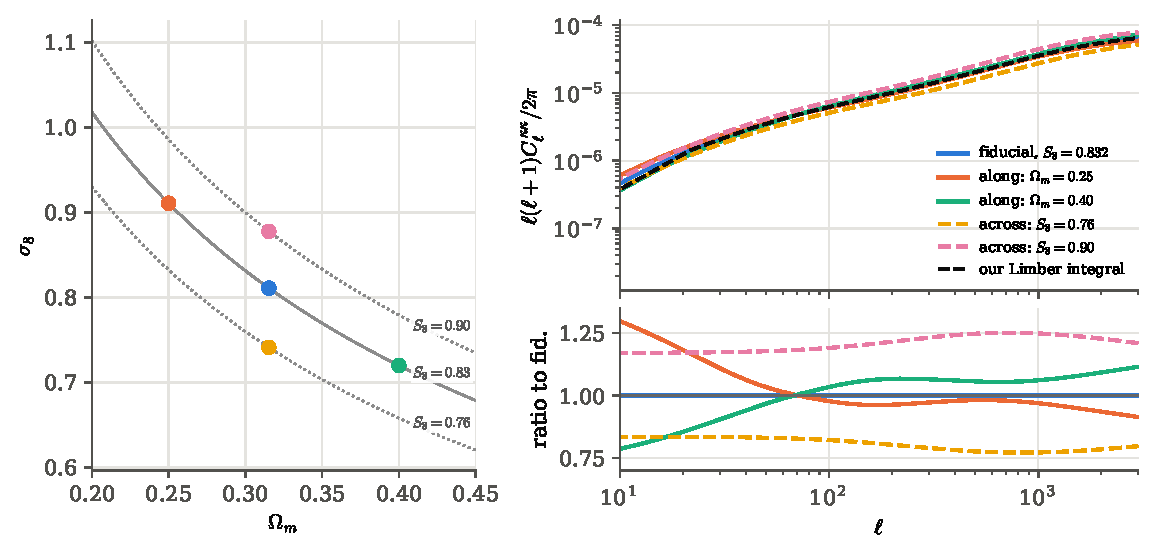
\includegraphics[width=\linewidth]{figures/chT1/kappa_s8_spectra.pdf}
\caption{Left: the five models in the $(\Omega_m,\sigma_8)$ plane, with lines of constant $S_8$. Right: their convergence spectra (top) and the ratio to the fiducial one (bottom). The three solid curves, on the fiducial $S_8$ line, stay close together for $\ell\gtrsim100$, even though $\Omega_m$ changes by a factor $1.6$ along it. The two dashed curves, off the line by about $9\%$ in $S_8$, are shifted by more than $20\%$ at every $\ell$. The dashed black curve is our own Limber integral for the fiducial model.}
\label{T1b:fig:s8}
\end{figure}

\subsection{The answer}
\label{T1b:sec:s8-answer}

\Cref{T1b:fig:s8} is the answer. Along the line of constant $S_8$ the spectra differ by a median of $\TOneAlongMedLo\%$ and $\TOneAlongMedHi\%$ over $100\le\ell\le2000$ (at most $\TOneAlongMax\%$), although $\Omega_m$ runs from $0.25$ to $0.40$ and $\sigma_8$ from $\TOneSigEightLo$ to $\TOneSigEightHi$. Across the line, a change of about $9\%$ in $S_8$ moves the spectrum by $\TOneAcrossLo\%$ and $\TOneAcrossHi\%$. So the data pin down $S_8$ and leave the position along the line almost free: for $\ell\gtrsim100$ the observation is about equally probable anywhere on the line, and the two candidates of the opening cannot be told apart there. Two things break that tie. A move across the line changes the spectrum by more than $20\%$, so the posterior is narrow in that direction. And at the low multipoles, $\ell\lesssim50$, the three solid curves separate.

Why at low $\ell$? The matter spectrum has a turnover, a peak at the wavenumber of the horizon size at matter--radiation equality, as described with the matter spectrum in \cref{T1a:sec:pk}. That wavenumber is $k_{\mathrm{eq}}\approx0.073\,\Omega_{m0}h^2\,\mathrm{Mpc}^{-1}$, which is $0.073\,\Omega_{m0}h$ in the units $h\,\mathrm{Mpc}^{-1}$ in which $\sigma_8$ is defined (see the cosmology notes). At fixed $h$ it moves in proportion to $\Omega_m$, by the factor $1.6$ between the ends of the line, and so the shape of $P_\delta$ around the turnover differs along the line even where its height does not. For the fiducial model $k_{\mathrm{eq}}\approx0.073\times0.315\times0.674^2\approx0.010\,\mathrm{Mpc}^{-1}$; matter near the peak of the lensing weight, at $\chi\approx1500$--$2000\,\mathrm{Mpc}$, projects it to $\ell=k\chi\approx15$--$20$. Only the lowest multipoles see the turnover, and they carry few modes.

\subsection{Which exponent?}
\label{T1b:sec:s8-alpha}

Is the exponent $0.5$ in $S_8$ special? We can ask the spectrum which exponent it prefers. Change $\Omega_m$ by $\pm5\%$ at fixed $\sigma_8$, then $\sigma_8$ by $\pm5\%$ at fixed $\Omega_m$, and form the logarithmic slopes. At $\ell=500$ they are $\partial\ln C_\ell/\partial\ln\sigma_8=\TOneDlnCdlnSEight$ and $\partial\ln C_\ell/\partial\ln\Omega_m=\TOneDlnCdlnOm$.

The first slope can be checked against what we know. In linear theory $C_\ell\propto\sigma_8^2$ at fixed $\Omega_m$, by \eqref{T1b:eq:cl-scaling}, so $\partial\ln C_\ell/\partial\ln\sigma_8=2$ exactly. Non-linear power grows faster than $\sigma_8^2$, because on small scales the extra clumping feeds on itself, and the measured $\TOneDlnCdlnSEight$ says how much faster: at $\ell=500$ the spectrum responds about $40\%$ more strongly than in linear theory. The same slope explains the across-line shifts of \cref{T1b:fig:s8}: $(0.76/0.832)^{2.8}-1=-22\%$ and $(0.90/0.832)^{2.8}-1=+25\%$, close to the measured $\TOneAcrossLo\%$ and $\TOneAcrossHi\%$, where the linear expectation of \cref{T1b:sec:s8-vary} was $\pm17\%$.

\emph{Which combination leaves the spectrum unchanged?} Write $a\equiv\partial\ln C_\ell/\partial\ln\sigma_8$ and $b\equiv\partial\ln C_\ell/\partial\ln\Omega_m$, and ask for the small changes of the two parameters that keep $C_\ell$ fixed:
\begin{align}
0=\dd\ln C_\ell
&\eqby{1}a\,\dd\ln\sigma_8+b\,\dd\ln\Omega_m
\quad\Longrightarrow\quad
\dd\ln\sigma_8\eqby{2}-\frac ba\,\dd\ln\Omega_m
\nonumber\\
\quad\Longrightarrow\quad
\ln\sigma_8+\frac ba\ln\Omega_m&\eqby{3}\text{const}
\quad\Longleftrightarrow\quad
\sigma_8\Omega_m^{b/a}=\text{const}.
\label{T1b:eq:alpha-derive}
\end{align}
\begin{explain}
  \item The change of a function of two variables is the sum of the changes along each (the chain rule), with $\ln\sigma_8$ and $\ln\Omega_m$ as the variables.
  \item Solve for $\dd\ln\sigma_8$.
  \item Integrate, treating the ratio $b/a$ as constant over the small region of interest; then take the exponential.
\end{explain}
The exponent is the ratio of the two slopes,
\begin{equation}
\alpha(\ell)\equiv\frac{\partial\ln C_\ell^{\kappa\kappa}/\partial\ln\Omega_m}{\partial\ln C_\ell^{\kappa\kappa}/\partial\ln\sigma_8}.
\label{T1b:eq:alpha}
\end{equation}
With the numbers above, $\alpha=\TOneDlnCdlnOm/\TOneDlnCdlnSEight\approx0.57$ at $\ell=500$, which the unrounded slopes give as $\TOneAlphaFive$. For the fiducial sample $\alpha=\TOneAlphaGalTwo$ at $\ell=200$, $\TOneAlphaFive$ at $\ell=500$ and $\TOneAlphaGalTwoK$ at $\ell=2000$.

\begin{figure}[htbp]
\centering
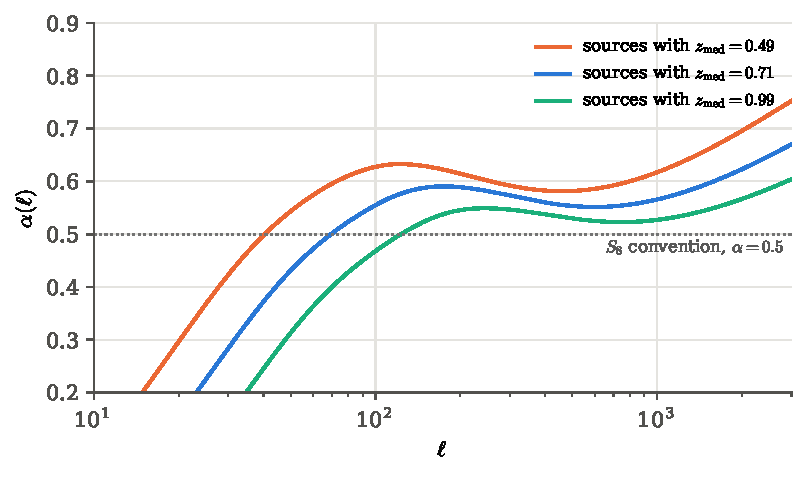
\includegraphics[width=0.8\linewidth]{figures/chT1/kappa_s8_alpha.pdf}
\caption{The exponent $\alpha$ of the combination $\sigma_8\Omega_m^\alpha$ that leaves $C_\ell^{\kappa\kappa}$ unchanged, multipole by multipole, \cref{T1b:eq:alpha}, for three source samples of increasing depth. Over the range where surveys have most of their signal, $100\lesssim\ell\lesssim1000$, it sits between $0.5$ and $0.6$, lower for deeper samples. It falls at low $\ell$, where the shape of the matter spectrum near its turnover enters.}
\label{T1b:fig:alpha}
\end{figure}

\Cref{T1b:fig:alpha} shows $\alpha(\ell)$ for three source samples, with median redshifts $\TOneZmedLo$, $\TOneZmed$ and $\TOneZmedHi$. At $\ell=500$ it is $\TOneAlphaLoFive$, $\TOneAlphaFive$ and $\TOneAlphaHiFive$. So the exponent $0.5$ is a convention close to the truth, not a law: the best exponent depends on the scales and the redshifts a survey uses. This is why the surveys quote their own. HSC finds its tightest combination at $\alpha=0.45$ and reports both $S_8(\alpha{=}0.45)=0.800^{+0.029}_{-0.028}$ and the standard $S_8=0.780^{+0.030}_{-0.033}$ \cite{Hikage2019HSC}, and CMB lensing, with its deeper kernel, measures $\sigma_8\Omega_m^{0.25}$ (\cref{T1b:sec:objects}).

\subsection{What the surveys find}
\label{T1b:sec:s8-surveys}

The question the surveys asked is simple to state. The CMB shows the Universe at $z\approx1100$, and the $\Lambda$CDM model extrapolates from it how clumpy matter should be today. Lensing measures today's clumpiness directly. \emph{Do the two agree?} Each experiment measures something different:
\begin{itemize}[leftmargin=1.2em,itemsep=1pt]
\item \emph{KiDS-1000} \cite{Asgari2021KiDS}: about $1000\,\mathrm{deg}^2$ ($777\,\mathrm{deg}^2$ effective), about $21$ million galaxies in five photometric bins out to $z\approx1.2$; its headline number comes from a two-point statistic of the shear in all fifteen bin pairs.
\item \emph{DES Year~3} \cite{Amon2022DES}: about $4100\,\mathrm{deg}^2$, about $100$ million galaxies in four bins, from the real-space correlations $\xi_\pm$.
\item \emph{HSC Year~1} \cite{Hikage2019HSC}: only $137\,\mathrm{deg}^2$ but the deepest images, four bins out to $z\approx1.5$, from tomographic power spectra $C_\ell^{ij}$.
\item \emph{Planck} \cite{Planck2018VI}: the CMB temperature and polarization spectra over the full sky, with $S_8$ today computed from the fitted $\Lambda$CDM parameters.
\end{itemize}

\begin{center}
\small
\begin{tabular}{@{}lccc@{}}
\toprule
experiment & published $S_8$ & symmetrised error & distance from Planck\\\midrule
KiDS-1000 & $0.759^{+0.024}_{-0.021}$ & $0.0225$ & $2.8\sigma$\\
DES Year~3 & $0.759^{+0.025}_{-0.023}$ & $0.024$ & $2.7\sigma$\\
HSC Year~1 & $0.780^{+0.030}_{-0.033}$ & $0.0315$ & $1.5\sigma$\\
Planck (CMB) & $0.832\pm0.013$ & $0.013$ & ---\\
this part & $\TOneSEightFid$; $0.76$, $0.90$ & --- & ---\\
\bottomrule
\end{tabular}
\end{center}

The distances in the last column are computed here, in one line of arithmetic. In the last row $\TOneSEightFid$ is the solid model of \cref{T1b:fig:s8} and $0.76$, $0.90$ the dashed ones. If the two measurements are independent and their errors Gaussian, their difference has a variance equal to the sum of the two variances, the rule behind \eqref{3a:eq:var-mean}, so for KiDS-1000
\[
\frac{0.832-0.759}{\sqrt{0.013^2+0.0225^2}}=\frac{0.073}{0.026}=2.8 .
\]
The ``about $3\sigma$'' that is often quoted is this number, rounded. It is only approximate: the errors are not symmetric (using the upper error, $0.024$, which is the one facing Planck, gives $2.7\sigma$), and the posteriors are not exactly Gaussian.

The sign of the shift is the one \cref{T1b:fig:s8} prepares. The lensing values sit near $S_8=0.76$, the lower dashed model, and the CMB value is the solid one: the surveys see a spectrum about $20\%$ below what Planck's $\Lambda$CDM predicts. Whether this is new physics, a nuisance not fully modelled (the red boxes of \cref{T1b:fig:pipeline}), or a fluctuation is one of the open questions of the field, and it is a question about statistics: about the sampling distribution of $\widehat C_\ell$, its covariance, and how much the nuisance parameters are allowed to move. The lesson of the comparison: a $9\%$ difference in one number is a $20\%$ difference in the spectrum, and whether it is significant depends entirely on errors that the later chapters learn to compute.

For the statistics chapters, the long valley of \cref{T1b:fig:s8} is a degeneracy of the kind met in \cref{T1a:sec:cl-response}: two parameters whose derivative curves are nearly proportional. In the Fisher matrix of \cref{ch:10} it makes the $(\Omega_m,\sigma_8)$ error ellipse long and thin, along $\sigma_8\Omega_m^\alpha=\text{const}$. In the MCMC of \cref{ch:09} it is a curved banana-shaped ridge. \Cref{ch:12} forecasts the error on $S_8$ from simulated maps and asks whether summaries beyond $C_\ell^{\kappa\kappa}$ shorten the banana.

\section{Experiment 2: signal and shape noise in a Stage-III survey}
\label{T1b:sec:noise}

The galaxy shapes carry a lensing signal of about $0.01$ under an intrinsic scatter of $0.27$. On which angular scales does the signal still win, and how many $\sigma$ is the whole detection worth? In the language of \cref{T1b:sec:objects}: $C_\ell^{ij}$ is the convergence spectrum between redshift bin $i$ and bin $j$, $N_i=\sigma_e^2/\bar n_i$ the shape-noise power of bin $i$ from \eqref{T1b:eq:shape-noise}, and the measured spectrum of bin $i$ is $C_\ell^{ii}+N_i$. We want to know where $C_\ell^{ii}$ exceeds $N_i$.

\subsection{The survey}
\label{T1b:sec:noise-survey}

We take survey numbers close to KiDS-1000 \cite{Asgari2021KiDS}:

\begin{center}
\small
\begin{tabular}{@{}lll@{}}
\toprule
quantity & this experiment & KiDS-1000\\\midrule
area & $\TOneArea\,\mathrm{deg}^2$ & $\approx1000\,\mathrm{deg}^2$ ($777\,\mathrm{deg}^2$ effective)\\
sky fraction $f_{\mathrm{sky}}$ & $\TOneFsky$ & ---\\
galaxy density $\bar n$ & $\TOneNeff$ arcmin$^{-2}$, all bins & $6.2$ arcmin$^{-2}$\\
shape scatter $\sigma_e$ (per component) & $\TOneSigmaE$ & $0.25$--$0.27$\\
photo-$z$ scatter & Gaussian, $0.05(1+z)$ & ---\\
redshift bins & $5$, equal numbers & $5$\\
\bottomrule
\end{tabular}
\end{center}

The sky fraction $f_{\mathrm{sky}}$ is the observed area divided by the area of the whole sky. The whole sky is $4\pi$ steradians, and one steradian is $(180/\pi)^2$ square degrees, so
\[
f_{\mathrm{sky}}=\frac{1000\,\mathrm{deg}^2}{4\pi(180/\pi)^2\,\mathrm{deg}^2}=\frac{1000}{41\,253}=\TOneFsky .
\]
The source sample is the one of \cref{T1b:sec:s8-fixed}, with the fiducial cosmology.

\subsection{The binning}
\label{T1b:sec:noise-bins}

We cut the sample into five bins by photometric redshift, with equal numbers of galaxies in each. Equal numbers make every bin equally noisy, since $N_i$ depends only on $\bar n_i$, so no bin is wasted on a handful of galaxies. A photometric redshift is estimated from a few broad colours, and its error grows with redshift because the spectral features it relies on are stretched by the factor $1+z$; the simplest model of that is a Gaussian scatter of width $0.05(1+z)$ about the true redshift, without the outliers that real catalogues have. The bin edges come out at $z_{\mathrm{ph}}=\TOneEdgeOne,\dots,\TOneEdgeFour$. Because of the scatter, a galaxy placed in one bin may truly belong to a neighbour, so the true-redshift distributions of the bins overlap.

\begin{figure}[htbp]
\centering
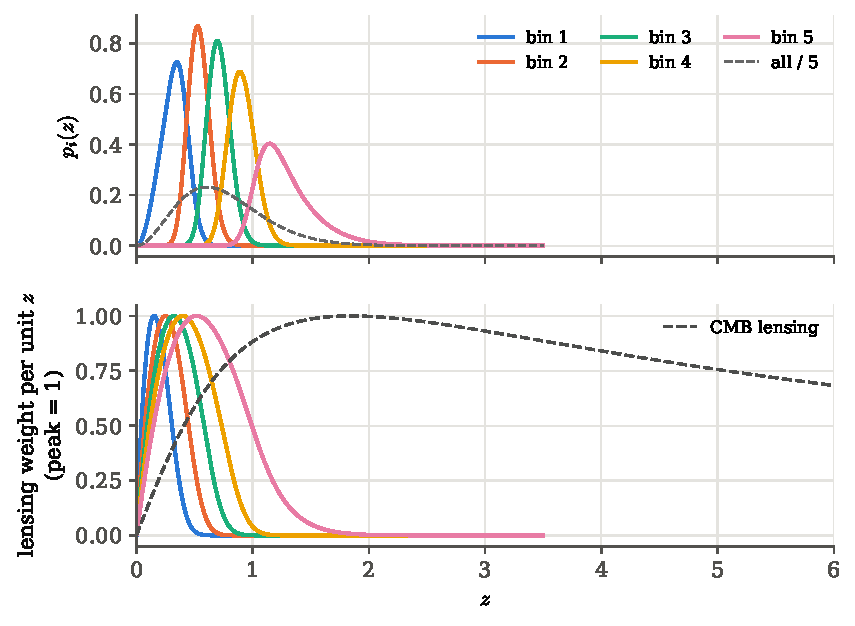
\includegraphics[width=0.78\linewidth]{figures/chT1/kappa_bins.pdf}
\caption{Top: the true-redshift distributions of the five photometric bins; photo-$z$ scatter makes them overlap. Bottom: the lensing weight of each bin per unit redshift, $\propto g_i(\chi)f_K(\chi)/a$ times $\dd\chi/\dd z$, normalised to peak at one. Each weight is broad and peaks at about half the distance of its sources, so the five bins see heavily overlapping slices of matter. The CMB weight (dashed) peaks near $z\approx2$.}
\label{T1b:fig:bins}
\end{figure}

\Cref{T1b:fig:bins} shows the price of photometric redshifts and of projection together. The bins themselves overlap, and their lensing weights overlap even more, since every bin is lensed by all the matter in front of it. Tomography therefore does not give five independent maps. It gives five correlated maps whose full $5\times5$ matrix of spectra, auto and cross, carries the information, and the covariance of the analysis must include all fifteen of them.

\subsection{The noise and the error bars}
\label{T1b:sec:noise-errors}

\pyfile[firstline=113,lastline=116,firstnumber=113]{code/chT1/04_kappa_noise.py}{The noise power of each bin}

Line~114 counts the fraction of galaxies in each bin (a fifth, by construction). Line~115 converts the number density from arcmin$^{-2}$ to sr$^{-1}$: one steradian holds $(10800/\pi)^2=1.18\times10^7$ arcmin$^2$, so $1.24$ arcmin$^{-2}$ becomes $1.47\times10^7\,\mathrm{sr}^{-1}$. Line~116 is the noise row of the table, $N_i=\sigma_e^2/\bar n_i\approx\TOneNoiseOne$, worked out in \cref{T1b:sec:objects}.

How large are the error bars on a measured band power? Start from the cosmic variance of one multipole and make three changes:
\begin{align}
\Var\widehat C_\ell
&\eqby{1}\frac{2C_\ell^2}{\nu}
\eqby{2}\frac{2\,(C_\ell+N)^2}{(2\ell+1)\,f_{\mathrm{sky}}},
&
\Var\Bigl(\frac1{\Delta\ell}\sum_{\ell'\in\text{band}}\widehat C_{\ell'}\Bigr)
&\eqby{3}\frac{2\,(C_\ell+N)^2}{(2\ell+1)\,\Delta\ell\,f_{\mathrm{sky}}},
\nonumber\\
\Delta C_\ell
&\eqby{4}\sqrt{\frac{2}{(2\ell+1)\,\Delta\ell\,f_{\mathrm{sky}}}}\,\bigl(C_\ell+N\bigr).
\label{T1b:eq:band-error}
\end{align}
\begin{explain}
  \item The cosmic variance \eqref{7b:eq:cosmic-var}, written for $\nu$ independent modes; on the full sky $\nu=2\ell+1$.
  \item Two changes. A survey that sees a fraction $f_{\mathrm{sky}}$ of the sky has only about $(2\ell+1)f_{\mathrm{sky}}$ independent modes per multipole. And what is measured is the spectrum of signal plus noise, whose variance per mode is $C_\ell+N$, so the scatter of the estimate is set by the sum, as in \eqref{7b:eq:cl-like-noise}; the noise is part of what is measured.
  \item Averaging the $\Delta\ell$ independent multipoles of a band divides the variance by $\Delta\ell$, \eqref{7b:eq:binned}, the variance of a mean.
  \item The square root.
\end{explain}
This is the Gaussian band-power error used in the literature \cite[eq.~52]{Kilbinger2015}.

What does this mean for inference? The observed band power is the model prediction plus one draw of noise with the variance of \eqref{T1b:eq:band-error}. Read as a function of the parameters $(\Omega_m,\sigma_8)$, the probability of the data asks how plausible the noise draw is that turns the prediction $C_\ell(\Omega_m,\sigma_8)$ into what was observed: a Gaussian centred on the model, with the width of \eqref{T1b:eq:band-error}. This is the likelihood from a noise model, \eqref{0a:eq:like-noise}, in its band-power form (\cref{7b:sec:cl-likelihood}). The $S_8$ degeneracy of \cref{T1b:sec:s8} is a statement about this likelihood: moving along the line leaves the centre almost where it was, so the same noise draw is needed everywhere on the line, and the likelihood does not change.

\begin{figure}[htbp]
\centering
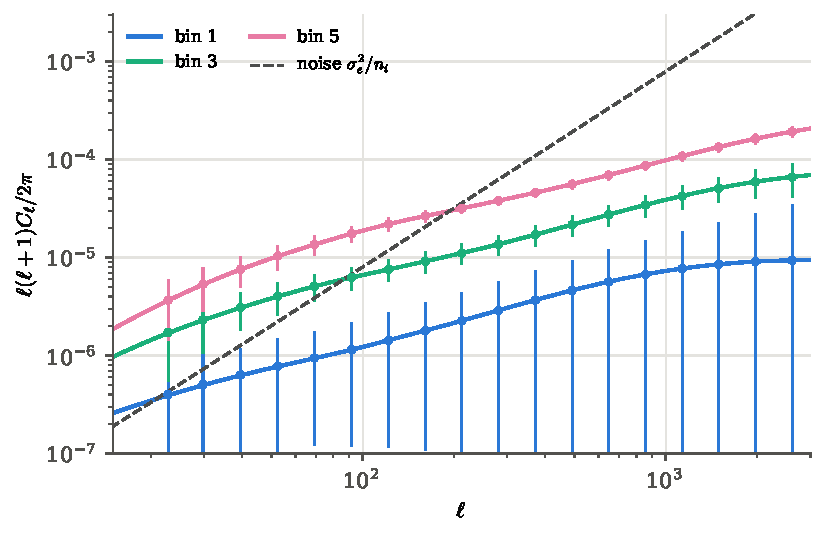
\includegraphics[width=0.8\linewidth]{figures/chT1/kappa_noise.pdf}
\caption{Convergence spectra of the nearest (1), middle (3) and farthest (5) bins, with Gaussian error bars on logarithmic bands of $\ell$ for a $1000\,\mathrm{deg}^2$ survey, \cref{T1b:eq:band-error}. The dashed line is the shape noise, the same for every bin because the bins hold equal numbers of galaxies; it rises as $\ell^2$ only because of the factor $\ell(\ell+1)$ on the axis. Beyond the crossing, the error bars are set mostly by the noise.}
\label{T1b:fig:noise}
\end{figure}

\subsection{Where the signal wins, and how many \texorpdfstring{$\sigma$}{sigma}}
\label{T1b:sec:noise-sn}

\Cref{T1b:fig:noise} gives the answer to the first question. The signal equals the noise at $\ell\approx\TOneLeqOne$ in the nearest bin, $\ell\approx\TOneLeqThree$ in the middle one and $\ell\approx\TOneLeqFive$ in the farthest, which is lensed by the most matter. Beyond those multipoles each bin is noise-dominated. The measurement does not stop there, since there are many modes at high $\ell$, but each additional mode adds little.

\emph{The signal-to-noise ratio of one bin.} Ask how well the data fix the height of the signal. Multiply the predicted spectrum by an amplitude $A$, so that the measured spectrum has mean $AC_\ell+N$, and define the signal-to-noise ratio as $1/\sigma(A)$ at $A=1$: the number of standard deviations by which the signal is distinguished from no signal. The Fisher information for $A$ comes from \eqref{10a:eq:cmb-fisher}, with $(2\ell+1)f_{\mathrm{sky}}$ modes per multipole:
\begin{align}
\Bigl(\frac SN\Bigr)^2
&\eqby{1}\sum_\ell\frac{(2\ell+1)f_{\mathrm{sky}}}{2}\,\frac{\bigl[\partial(AC_\ell+N)/\partial A\bigr]^2}{(C_\ell+N)^2}
\eqby{2}\sum_\ell\frac{(2\ell+1)f_{\mathrm{sky}}}{2}\,\frac{C_\ell^2}{(C_\ell+N)^2}.
\label{T1b:eq:sn-one}
\end{align}
\begin{explain}
  \item \Cref{10a:eq:cmb-fisher} for one parameter, with the full-sky count $2\ell+1$ replaced by $(2\ell+1)f_{\mathrm{sky}}$, and the inverse error squared equal to the Fisher information.
  \item The derivative of $AC_\ell+N$ with respect to $A$ is $C_\ell$.
\end{explain}
Each mode contributes the factor $\frac12[C_\ell/(C_\ell+N)]^2$. Where the signal dominates, $C_\ell\gg N$, that factor is $\frac12$, the most a mode can give; where the noise dominates it falls as $\frac12(C_\ell/N)^2$, and since $N$ is flat while $C_\ell$ falls, it drops quickly beyond the crossing. So the signal-to-noise ratio essentially counts the modes below the crossing multipole.

\emph{Five bins at once.} With tomography the spectrum at each $\ell$ is a $5\times5$ matrix $\mathbf C_\ell$ with entries $C_\ell^{ij}+\delta_{ij}N_i$, and $\mathbf S_\ell$ is its signal part. The same calculation with the matrix form of the Fisher information gives
\begin{equation}
\Bigl(\frac SN\Bigr)^2=\sum_\ell\frac{(2\ell+1)f_{\mathrm{sky}}}{2}\,\Tr\bigl[\mathbf C_\ell^{-1}\mathbf S_\ell\,\mathbf C_\ell^{-1}\mathbf S_\ell\bigr],
\label{T1b:eq:sn-tomo}
\end{equation}
which for one bin reduces to \eqref{T1b:eq:sn-one}. The fifteen distinct spectra are the entries of $\mathbf S_\ell$, and the inverse $\mathbf C_\ell^{-1}$ accounts for the correlations between bins that \cref{T1b:fig:bins} shows, so that shared information is not counted twice. Summing over $10\le\ell\le\TOneLmaxSN$, the total signal-to-noise ratio is $\TOneSNtomo$. A single unbinned sample, with five times the galaxies and so a fifth of the noise, gives $\TOneSNone$. The ratio is $\TOneSNtomo/\TOneSNone\approx1.14$: tomography adds about $14\%$ to the detection. What it buys is the redshift dependence, which separates the growth of structure from the geometry and helps tell intrinsic alignments from lensing.

\emph{How well is the amplitude measured?} If $\sigma_8$ were the only unknown, the Fisher information on $\ln\sigma_8$ is \eqref{T1b:eq:sn-tomo} with each $\mathbf S_\ell$ replaced by the derivative $\partial\mathbf C_\ell/\partial\ln\sigma_8$ (the general form is \eqref{10a:eq:gauss-fisher}), and with a single parameter the error is $\sigma(\ln\sigma_8)=1/\sqrt F$. The derivative comes from two more CAMB runs at $\sigma_8(1\pm\epsilon)$ with $\epsilon=0.02$, as a central difference (\cref{10a:sec:numderiv}):
\[
\frac{\partial\mathbf C_\ell}{\partial\ln\sigma_8}\approx\frac{\mathbf C_\ell^{+}-\mathbf C_\ell^{-}}{\ln(1+\epsilon)-\ln(1-\epsilon)}\approx\frac{\mathbf C_\ell^{+}-\mathbf C_\ell^{-}}{2\epsilon}.
\]
The result is $\sigma(\ln\sigma_8)=\TOneSigLnSEight\%$. It can be checked against the signal-to-noise ratio. If the derivative were a fixed multiple $s$ of the signal, $\partial\mathbf C_\ell/\partial\ln\sigma_8=s\,\mathbf S_\ell$, then $F=s^2(S/N)^2$ and $\sigma(\ln\sigma_8)=1/[s\,(S/N)]$. In linear theory $s=2$, giving $1/(2\times\TOneSNtomo)=1.0\%$. The computed $\TOneSigLnSEight\%$ corresponds to $s\approx1/(0.008\times\TOneSNtomo)\approx2.6$, between the linear $2$ and the $\TOneDlnCdlnSEight$ found at $\ell=500$ in \cref{T1b:sec:s8-alpha}: the non-linear boost again.

At fixed $\Omega_m$ this is also the error on $S_8$. KiDS-1000 achieves about $3\%$. The gap between the two numbers is the content of the later chapters. The first cost can be sized here. $\Omega_m$ is free and degenerate with $\sigma_8$ (\cref{T1b:sec:s8}). For two parameters with Fisher matrix entries $F_{\sigma\sigma}$, $F_{\Omega\Omega}$ and $F_{\sigma\Omega}$,
\begin{align}
\sigma^2_{\text{marg}}(\ln\sigma_8)
&\eqby{1}\bigl(F^{-1}\bigr)_{\sigma\sigma}
\eqby{2}\frac{F_{\Omega\Omega}}{F_{\sigma\sigma}F_{\Omega\Omega}-F_{\sigma\Omega}^2}
\eqby{3}\frac{1}{F_{\sigma\sigma}}\,\frac{1}{1-r^2},
\qquad r\equiv\frac{F_{\sigma\Omega}}{\sqrt{F_{\sigma\sigma}F_{\Omega\Omega}}}.
\label{T1b:eq:marg-cost}
\end{align}
\begin{explain}
  \item The marginal error is read from the inverse of the Fisher matrix (\cref{10a:sec:degeneracy}).
  \item The inverse of a $2\times2$ matrix.
  \item Divide the numerator and the denominator by $F_{\sigma\sigma}F_{\Omega\Omega}$; $r$ is the cosine of the angle between the two derivative curves, weighted as in the Fisher sum.
\end{explain}
So freeing $\Omega_m$ multiplies the error on $\ln\sigma_8$ by $1/\sqrt{1-r^2}$: by $2.3$ for $r=0.9$ and by $7$ for $r=0.99$, and the near-proportional derivative curves of \cref{T1b:sec:s8} put $r$ close to one. The combination $S_8$ is chosen to lie along the well-measured direction, so its error grows much less, which is why the surveys quote it. The rest of the gap comes from the other costs. Nuisance parameters for photo-$z$ shifts, shear bias, intrinsic alignment and baryons are marginalised. The covariance has non-Gaussian and super-sample terms that \cref{T1b:eq:band-error} ignores. And the smallest scales are cut because baryonic feedback is uncertain there. \Cref{ch:10} computes each of these costs in the Fisher matrix, and \cref{ch:12} redoes the forecast with simulated maps.

\begin{inpractice}[What the full analysis does]
Our numbers come from a Gaussian, nuisance-free forecast with all other parameters fixed. The published analyses measure tomographic $\xi_\pm(\vartheta)$, band powers or related statistics from tens of millions of shapes \cite{Asgari2021KiDS,Amon2022DES,Hikage2019HSC}. They take the covariance from analytic models checked against hundreds to thousands of ray-traced $N$-body simulations, such as the full-sky lensing maps of \cite{Takahashi2017sims}, and they sample the posterior of cosmological and nuisance parameters by MCMC. The same simulations are what make summaries beyond two-point statistics usable: peak counts \cite{Kratochvil2010,DietrichHartlap2010}, Kaiser--Squires mass maps \cite{Jeffrey2021DESmass}, lognormal fields as a fast model of the skewed $\kappa$ distribution \cite{Xavier2016}, and persistent homology of $\kappa$ maps \cite{Heydenreich2021}. All of these return in \cref{ch:12}.
\end{inpractice}

The lesson of the two experiments for the rest of the book is in two parts. The signal is a projected, smoothed field whose two-point statistic is degenerate along $S_8$. The noise is white, large and known. So the statistical problem is to extract as much as possible from a noisy, non-Gaussian field with a small number of summaries. \Cref{ch:12} takes up that problem with topological summaries.

\begin{recap}
\begin{itemize}[leftmargin=1.2em,itemsep=1pt]
\item Lensing distorts galaxy images by about $1\%$: $\kappa=\frac12\nabla^2\psi$ magnifies, the spin-2 shear $\gamma_1=\frac12(\psi_{,11}-\psi_{,22})$, $\gamma_2=\psi_{,12}$ stretches; a galaxy measures $\varepsilon\approx\varepsilon^{(0)}+\gamma$, with the reduced shear $\gamma/(1-\kappa)$ as its mean.
\item Lensing makes only $E$ modes; a $B$ mode is a null test for systematics.
\item $C_\ell^{\kappa\kappa}$ is the Limber integral of $[g/a]^2P_\delta$ over distance, with the broad lensing efficiency $g(\chi)$; CAMB computes it with lensing source windows, and our own integral agrees to $\TOneLimberErr\%$.
\item Cosmic shear measures $\sigma_8\Omega_m^\alpha$ with $\alpha\approx\TOneAlphaFive$ for a Stage-III sample ($S_8$ takes $\alpha=0.5$); along that line the spectrum changes by a few per cent, across it by $\sim20\%$ for a $9\%$ change in $S_8$.
\item Shape noise $N_i=\sigma_e^2/\bar n_i$ is white; for a KiDS-like survey the signal beats it only up to $\ell\approx\TOneLeqOne$--$\TOneLeqFive$ per bin; total $S/N\approx\TOneSNtomo$, $\sigma(\ln\sigma_8)=\TOneSigLnSEight\%$ with everything else fixed, against $\approx3\%$ achieved with nuisances marginalised.
\item Nuisances: photo-$z$ shifts, shear bias $m$, intrinsic alignments, baryonic feedback. CMB lensing ($\psi$ reconstructed by a quadratic estimator) weights $z\approx2$ and measures $\sigma_8\Omega_m^{0.25}$.
\end{itemize}
\end{recap}

\section*{Chapter summary}
\addcontentsline{toc}{section}{Chapter summary}
\label{T1a:sec:summary}

The cosmological model is the first step of the book's pipeline. For every choice of the six $\Lambda$CDM numbers it fixes the expected value of each summary that the later chapters estimate from data, and never the sky itself. The route is short enough to hold in the head. The Friedmann equation gives the expansion rate $E(z)$, and one integral of $1/E$ gives the distances $D_A$ and $D_L$. The primordial spectrum $\mathcal P_\zeta=A_s(k/k_*)^{n_s-1}$ is carried to the sky by the radiation transfer function, $C_\ell=\frac2\pi\int k^2\dd k\,P_\zeta\,g_{T\ell}^2$, and to the matter field by growth and the matter transfer function, $P_\delta(k,a_0)=P_\delta(k,a_{\mathrm i})\,T^2[D_+(a_0)/D_+(a_{\mathrm i})]^2$. The data are one draw from each: the $\alm$ with variance $\Cell$, the Fourier modes $\delta_{\bm k}$ with variance $P_\delta(k)$. Weak lensing adds a third field built from the same matter: projected along the line of sight with the lensing efficiency $g(\chi)$, it becomes the convergence $\kappa$, whose power spectrum $C_\ell^{\kappa\kappa}$ is a Limber integral of $P_\delta$, and it is read off galaxy shapes through the shear $\gamma$, buried under shape noise.

What carries into the inference chapters is how these predictions move when the parameters move. The finite-difference responses $R_i(\ell)$ of \cref{T1a:eq:response} are the derivatives of the Fisher matrix, two nearly parallel responses are a degeneracy, and the line between linear and halofit $P(k)$ is where the Gaussian description of the matter field stops. Conventions are the fixed factors that decide whether a script reproduces these numbers. The table lists what to carry forward, what each item means in practice, and where it is used.

\begin{center}
\small
\renewcommand{\arraystretch}{1.15}
\begin{tabularx}{\linewidth}{@{}>{\raggedright\arraybackslash}p{3.3cm}
                               >{\raggedright\arraybackslash}X
                               >{\raggedright\arraybackslash}p{2.4cm}@{}}
\toprule
concept & operational meaning & used later in\\\midrule
model as a machine & six numbers into CAMB, expected statistics out; call it through \pyname{code/camb_fiducial.py} for the fiducial spectra & \cref{ch:07,ch:08,ch:09,ch:10}\\
one realisation & the sky is one draw; each $\alm$ has variance $\Cell$, and $\widehat C_\ell$ scatters about $\Cell$ as $\chi^2_{2\ell+1}/(2\ell+1)$ & \cref{ch:07,ch:08}\\
distances and $H(z)$ & $E(z)$ from the density parameters, then $D_A$, $D_L$ by one integral; the model mean of supernova and BAO data & \cref{ch:03,ch:05}\\
conventions & raw $\Cell$ vs $D_\ell$; $\mu\mathrm K^2$; $A_s=\frac{25}{4}A_S^2$; $h^{-1}$Mpc; $\phi\equiv\psi$ & every CMB and LSS script\\
fractional response $R_i(\ell)$ & central difference of $\Cell$ over $\pm1\sigma$, divided by $2\Cell$; times $\Cell/\delta_i$ it is $\partial\Cell/\partial\theta_i$ & \cref{ch:10}\\
degeneracy & two nearly parallel response curves ($A_s$ and $\tau$ above $\ell\approx30$); a near-singular Fisher matrix and a ridge in the chain & \cref{ch:09,ch:10}\\
linear vs halofit $P(k)$ & agree on large scales, differ by $10\%$ at $k\approx\TOneKnl\,h\,\mathrm{Mpc}^{-1}$ at $z=0$; beyond that the field is non-Gaussian & \cref{ch:07,ch:12}\\
$\xi(r)$ and the BAO bump & Fourier partner of $P(k)$; a peak near $r_s(z_{\mathrm{drag}})$, a standard ruler & \cref{ch:07,ch:12}\\
$\sigma_8$ & top-hat variance of the linear field at $8\,h^{-1}$Mpc; a check that $P(k)$ is normalised correctly & \cref{ch:07,ch:10}\\
$f_{\mathrm{NL}}$ & amplitude of the primordial bispectrum; invisible to $\Cell$ and $P(k)$ & \cref{ch:12}\\
$\kappa$, $\gamma$, $E$/$B$ & projected density and its spin-2 tidal stretch (\cref{T1b:sec:shapes}); lensing makes only $E$, so $B$ is a null test & \cref{ch:12}\\
$C_\ell^{\kappa\kappa}$ and shape noise & Limber integral of $[g/a]^2P_\delta$ (CAMB lensing windows); measured power $C_\ell^{ij}+\delta_{ij}\sigma_e^2/\bar n_i$ & \cref{ch:10,ch:12}\\
$S_8$ and nuisances & cosmic shear fixes $\sigma_8\Omega_m^{\alpha}$, $\alpha\approx0.55$; photo-$z$, shear bias, intrinsic alignment, baryons are marginalised & \cref{ch:09,ch:10,ch:12}\\
\bottomrule
\end{tabularx}
\end{center}

\paragraph{Reading the literature.}
The physics of every object above is developed in the cosmology notes. The Boltzmann code used throughout is CAMB \cite{CAMB2000}. The parameter values and errors are those of Planck 2018 \cite{Planck2018VI}. The non-linear correction is the halofit version of \cite{Takahashi2012}, and the first detection of the BAO bump in the galaxy correlation function is \cite{Eisenstein2005}. For weak lensing, the standard reviews are \cite{BartelmannSchneider2001} and \cite{Kilbinger2015}, CMB lensing is reviewed in \cite{LewisChallinor2006} and measured in \cite{Planck2018VIII}, and the Stage-III cosmic-shear results are \cite{Asgari2021KiDS,Amon2022DES,Hikage2019HSC}.
 